\documentclass[12pt,a4paper]{report}
\pdfminorversion=7
\usepackage[T1]{fontenc}
\usepackage[utf8]{inputenc}
\usepackage[italian]{babel}
\usepackage{amsmath,amssymb,amsthm}
\usepackage[a4paper,left=3cm,right=2cm,top=2.5cm,bottom=2.5cm]{geometry}
\usepackage{graphicx}
\usepackage{float}
\usepackage{hyperref}
\usepackage{pdfpages}
\usepackage{enumitem}
\usepackage{indentfirst}
\usepackage{matlab-prettifier}
\usepackage{ragged2e}
\usepackage{booktabs}
\usepackage{xcolor}
\usepackage{setspace}

\lstset{language=Matlab,
basicstyle=\ttfamily\footnotesize,
columns=fullflexible
}

\setlist[enumerate,1]{label=(\alph*), leftmargin=1.2cm, rightmargin=1.2cm}
\renewcommand{\contentsname}{Indice dei contenuti}
\renewcommand{\figurename}{Figura}
\setlength{\parindent}{1cm}
\setlength{\parskip}{0pt}
\onehalfspacing

\title{Elaborazione e aggregazione di dati privacy-aware con tecniche omomorfiche}
\author{Doru Ionut Parvu}
\date{}

\begin{document}

\pagestyle{plain}
\justifying
\hypersetup{pageanchor=false}
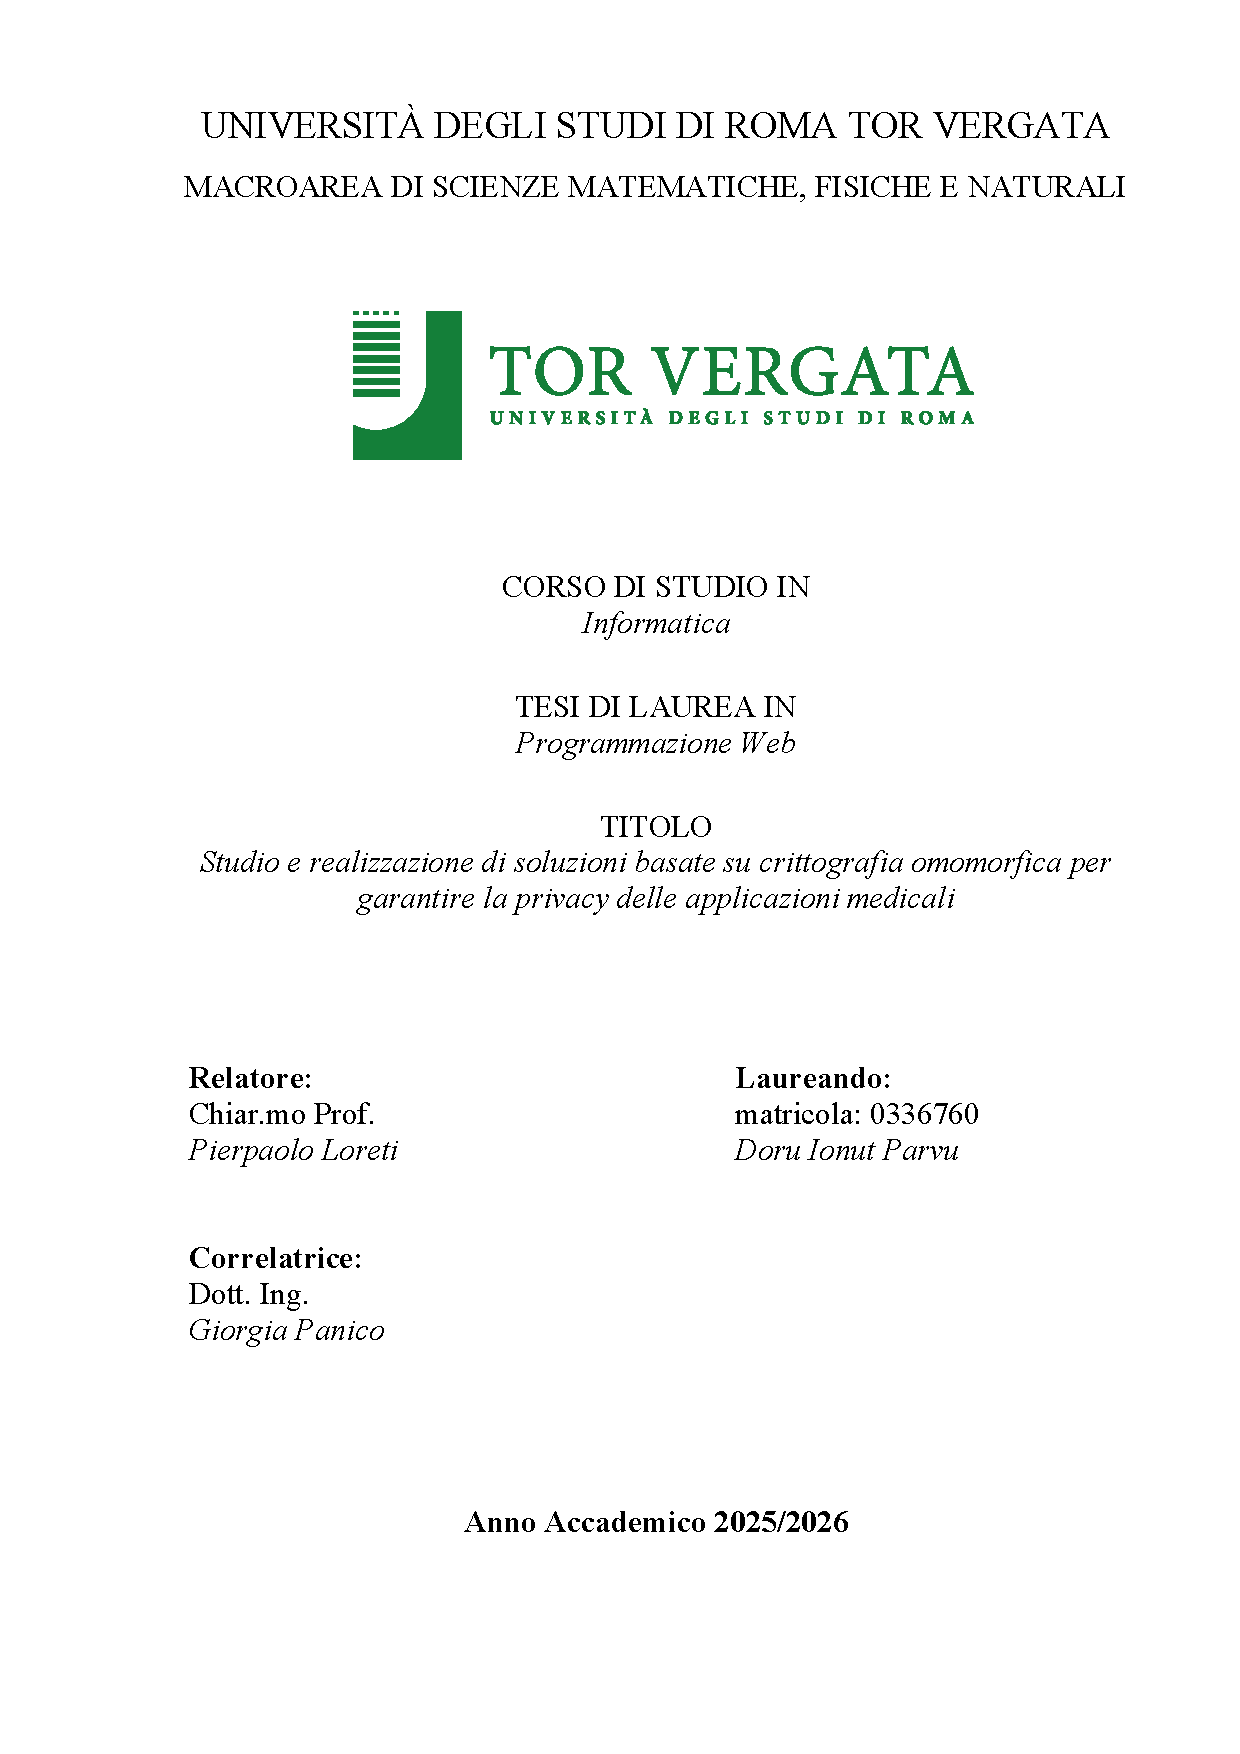
\includepdf[pages=1,pagecommand={\thispagestyle{empty}}]{frontespizio.pdf}
\clearpage
\hypersetup{pageanchor=true}
\pagenumbering{roman}
\tableofcontents
\clearpage
\pagenumbering{arabic}

\chapter{Introduzione}

\section{Contesto e motivazione}
La quantit\`a di dati raccolti da organizzazioni pubbliche e private cresce continuamente. Ospedali, centri di ricerca, aziende e servizi digitali producono informazioni che possono essere utili per costruire modelli statistici, calcolare indicatori o conoscere l'andamento di un fenomeno. Molti di questi dati sono per\`o sensibili. Un dato medico, una misura economica o una preferenza personale non dovrebbe essere consegnata in chiaro a ogni soggetto che partecipa all'elaborazione.

La soluzione pi\`u immediata consiste nel cifrare i dati quando vengono salvati o trasmessi. La cifratura tradizionale protegge bene queste due fasi, ma normalmente richiede di decifrare le informazioni prima di elaborarle. Il server che esegue il calcolo torna quindi a vedere i valori originali. Questo passaggio crea un punto delicato: per ottenere un risultato bisogna concedere fiducia all'infrastruttura che esegue il calcolo.

La cifratura omomorfica affronta il problema da una prospettiva diversa. Essa permette di eseguire alcune operazioni direttamente sui dati cifrati. Il server riceve ciphertext, cio\`e rappresentazioni non leggibili, applica somme o moltiplicazioni e produce un nuovo ciphertext. Dopo la decifratura, il risultato corrisponde al calcolo che sarebbe stato eseguito sui dati in chiaro. Il server pu\`o quindi contribuire all'elaborazione senza conoscere necessariamente gli input.

Questa propriet\`a \`e interessante, ma non rende il calcolo cifrato gratuito o automaticamente adatto a ogni applicazione. Le operazioni omomorfiche sono pi\`u lente delle operazioni ordinarie, richiedono pi\`u memoria e dipendono da parametri che devono essere scelti con attenzione. Schemi diversi rappresentano tipi di dato diversi e offrono compromessi differenti tra precisione, capacit\`a di calcolo e costo.

\section{Obiettivo della tesi}
L'obiettivo di questa tesi \`e studiare in modo progressivo come le tecniche omomorfiche possano essere usate per elaborare e aggregare dati proteggendo maggiormente i contributi individuali. Il lavoro non si limita a descrivere gli schemi da un punto di vista teorico. La parte centrale consiste nel collegare le loro caratteristiche a misure sperimentali e, successivamente, a due applicazioni concrete.

Le domande che guidano il lavoro sono semplici:
\begin{itemize}
  \item quali tipi di dato possono essere rappresentati dai principali schemi omomorfici;
  \item quali parametri incidono maggiormente sul costo delle operazioni;
  \item quale differenza pratica esiste tra sommare e moltiplicare dati cifrati;
  \item come usare queste tecniche in un modello di regressione lineare;
  \item come costruire un protocollo di aggregazione ispirato alle VDAF, nel quale il risultato collettivo possa essere recuperato senza trattare in chiaro ogni contributo.
\end{itemize}

La tesi considera tre schemi disponibili nella libreria OpenFHE: BFV, BGV e CKKS. BFV e BGV sono adatti a operazioni esatte su interi rappresentati in uno spazio modulare. CKKS \`e invece progettato per calcoli approssimati su valori reali o complessi ed \`e quindi utile per molte elaborazioni statistiche e di machine learning \cite{openfhe,ckks}.

\section{Percorso seguito}
Il lavoro \`e iniziato dallo studio tecnologico degli schemi omomorfici. Prima di scegliere uno schema per un'applicazione, \`e infatti necessario capire che cosa possa rappresentare, quali operazioni supporti e come cambino i ciphertext durante il calcolo. Particolare attenzione \`e stata dedicata alla dimensione dell'anello, al numero di slot disponibili, al modulo del plaintext e alla profondit\`a moltiplicativa.

Il secondo passo \`e stato la costruzione di una suite di benchmark basata su OpenFHE. Gli esperimenti misurano il tempo di creazione del contesto, la generazione delle chiavi, la cifratura, la decifratura, la somma e la moltiplicazione omomorfiche. Per CKKS sono stati misurati anche la generazione delle chiavi di bootstrapping e il bootstrapping stesso. I test variano la dimensione dell'anello e la profondit\`a richiesta, in modo da osservare come aumentino tempo e memoria.

I benchmark non servono a dichiarare uno schema vincitore in ogni situazione. Il loro scopo \`e mostrare che la scelta dipende dal problema. Se i dati sono conteggi interi e si desiderano risultati esatti, BFV o BGV sono candidati naturali. Se si elaborano medie, coefficienti o misure non intere, CKKS offre una rappresentazione pi\`u adatta, accettando un piccolo errore numerico.

Dopo il confronto sperimentale, il lavoro applica CKKS a un caso di machine learning semplice e interpretabile: la regressione lineare. Il caso di studio usa dati sanitari e stima la durata di un ricovero. La regressione \`e stata scelta perch\'e permette di osservare con chiarezza il passaggio dai dati cifrati al modello e perch\'e l'inferenza richiede principalmente somme e moltiplicazioni.

L'ultima parte si sposta dal machine learning all'aggregazione verificabile. Viene presentato un protocollo ispirato a VDAF Prio3, ma reinterpretato tramite BGV. I client cifrano report interi, l'aggregatore verifica sotto cifratura che la loro rappresentazione sia valida e somma i contributi accettati. Il collector decifra il totale finale. L'obiettivo non \`e riprodurre integralmente Prio3, ma studiare una costruzione pi\`u semplice che mantenga l'idea di apprendere un aggregato senza esporre direttamente ogni report.

\section{Contributi principali}
I contributi del lavoro possono essere riassunti in quattro punti.

\begin{enumerate}
  \item Una descrizione accessibile delle caratteristiche operative di BFV, BGV e CKKS, con una distinzione tra limiti dello schema, limiti della libreria e limiti della configurazione scelta.
  \item Una suite sperimentale comune per confrontare le principali operazioni omomorfiche al variare della dimensione dell'anello e della profondit\`a moltiplicativa.
  \item Un'applicazione di CKKS alla regressione lineare in uno scenario sanitario, con due possibili distribuzioni dei ruoli di calcolo e decifratura.
  \item Una costruzione di aggregazione VDAF-like basata su BGV, con codifica binaria, validazione omomorfica e decifratura del solo risultato aggregato.
\end{enumerate}

Il filo comune \`e il passaggio dalla singola operazione crittografica a un sistema completo. La scelta dello schema influenza il formato dei dati; i parametri influenzano costo e capacit\`a; l'architettura stabilisce quali attori possano cifrare, calcolare e decifrare. La privacy non dipende quindi da un solo algoritmo, ma dall'insieme di queste decisioni.

\section{Conclusioni}
La cifratura omomorfica permette di ripensare il rapporto tra dati e calcolo: il soggetto che elabora non deve necessariamente vedere ci\`o che elabora. Questa possibilit\`a apre scenari utili, ma introduce costi e vincoli che devono essere misurati e compresi.

La tesi segue quindi un percorso intenzionalmente graduale. Parte dagli strumenti di base, li misura, li applica a un modello statistico e infine li inserisce in un protocollo di aggregazione. In questo modo teoria, benchmark e applicazioni non restano parti separate, ma descrivono fasi successive dello stesso problema.

\chapter{Tecniche di cifratura omomorfica}

\section{Calcolare senza decifrare}
In una cifratura tradizionale un mittente trasforma un messaggio leggibile in un ciphertext usando una chiave. Chi possiede la chiave corretta pu\`o recuperare il messaggio originale. Se il dato deve essere elaborato, normalmente viene prima decifrato.

La cifratura omomorfica aggiunge una possibilit\`a: alcune operazioni possono essere eseguite direttamente sui ciphertext. Si pu\`o immaginare un'azienda che voglia conoscere la somma delle vendite di pi\`u negozi senza leggere il valore di ciascun negozio. Ogni sede cifra il proprio dato; il server somma i ciphertext; il soggetto autorizzato decifra soltanto il totale.

Un sistema di questo tipo comprende normalmente:
\begin{itemize}
  \item una fase di configurazione, nella quale vengono scelti schema e parametri;
  \item la generazione di una chiave pubblica e di una chiave segreta;
  \item eventuali chiavi di valutazione, necessarie per operazioni come moltiplicazioni e rotazioni;
  \item la codifica e la cifratura dei dati;
  \item la valutazione omomorfica;
  \item la decifratura e la decodifica del risultato.
\end{itemize}

La chiave pubblica pu\`o essere distribuita ai soggetti che devono cifrare. La chiave segreta deve invece restare presso il soggetto autorizzato a leggere il risultato. Le chiavi di valutazione consentono al server di trasformare i ciphertext durante il calcolo, ma non dovrebbero permettergli di recuperarne il contenuto.

\section{Base tecnologica: reticoli e rumore}
Gli schemi considerati in questa tesi si basano su problemi matematici legati ai reticoli. Per comprendere il funzionamento operativo non \`e necessario studiare la geometria completa di questi oggetti. \`E sufficiente osservare che un ciphertext contiene il messaggio in una forma nascosta insieme a una componente casuale, spesso chiamata rumore.

Il rumore \`e utile per la sicurezza, perch\'e impedisce di riconoscere direttamente il messaggio. Durante le operazioni omomorfiche, tuttavia, anche il rumore cambia. Le somme lo aumentano in modo generalmente contenuto; le moltiplicazioni hanno un effetto molto maggiore. Se il rumore supera il margine previsto dai parametri, la decifratura pu\`o restituire un valore errato.

Per questo motivo il programma da eseguire deve essere considerato prima di creare il contesto crittografico. Non basta sapere quanti dati saranno cifrati: bisogna conoscere soprattutto quante moltiplicazioni consecutive saranno necessarie. Questo valore \`e chiamato profondit\`a moltiplicativa.

\subsection{Leveled FHE e bootstrapping}
Un sistema \emph{leveled} viene configurato per sostenere una profondit\`a massima. Se il calcolo resta entro quel limite, non \`e necessario rinnovare il ciphertext. BGV ha reso particolarmente importante questa impostazione, mostrando come eseguire circuiti di profondit\`a prefissata senza ricorrere obbligatoriamente al bootstrapping \cite{bgv}.

Il bootstrapping \`e un'operazione pi\`u complessa che riduce l'effetto del rumore e rende nuovamente utilizzabile un ciphertext vicino al proprio limite. Permette di proseguire calcoli pi\`u lunghi, ma richiede chiavi aggiuntive, memoria e molto pi\`u tempo rispetto a una somma o a una singola moltiplicazione. In pratica si preferisce evitarlo quando il calcolo pu\`o essere dimensionato in anticipo.

\section{Dati inseriti negli slot}
I ciphertext moderni non devono necessariamente contenere un solo numero. Attraverso il \emph{packing}, pi\`u valori vengono inseriti in posizioni chiamate slot. Una singola operazione pu\`o quindi agire contemporaneamente su molti elementi, secondo un modello simile al SIMD: la stessa istruzione viene applicata in parallelo a pi\`u dati.

Se due ciphertext contengono rispettivamente i vettori
\[
[2,4,6,8]
\qquad\text{e}\qquad
[1,3,5,7],
\]
la loro somma omomorfica produce un ciphertext che, una volta decifrato, contiene
\[
[3,7,11,15].
\]
Il costo dell'operazione non cresce come se fossero state eseguite quattro cifrature separate. Il packing \`e quindi essenziale per rendere pratiche aggregazioni e operazioni vettoriali.

\subsection{Dimensione dell'anello e numero di slot}
La \emph{ring dimension}, indicata spesso con $N$, \`e uno dei parametri centrali. Una dimensione maggiore pu\`o offrire pi\`u slot e sostenere parametri crittografici pi\`u grandi, ma aumenta anche la dimensione dei ciphertext, il tempo delle operazioni e il consumo di memoria.

Nell'implementazione di benchmark usata in questa tesi, BFV e BGV impiegano fino a $N$ slot con il packed encoding, mentre CKKS utilizza $N/2$ slot complessi.

Una dimensione maggiore non significa automaticamente maggiore efficienza. Se l'applicazione usa pochi valori, gran parte degli slot rimane vuota mentre il costo del ciphertext resta elevato. Il vantaggio emerge quando gli slot vengono riempiti con un batch abbastanza grande.

\subsection{Rotazioni}
Le somme e le moltiplicazioni agiscono slot per slot. Per combinare elementi che occupano posizioni diverse servono le rotazioni. Una rotazione sposta ciclicamente il contenuto degli slot; ripetendo rotazioni e somme si pu\`o, ad esempio, calcolare la somma di tutti gli elementi di un vettore.

Le rotazioni richiedono evaluation keys dedicate. Generare e conservare molte chiavi di rotazione pu\`o avere un costo rilevante. Una buona disposizione dei dati negli slot riduce il numero di rotazioni richieste e pu\`o incidere sull'efficienza quanto la scelta dello schema.

\section{BFV e BGV: interi esatti modulo un primo}
BFV, derivato dal lavoro di Fan e Vercauteren \cite{bfv}, e BGV \cite{bgv} rappresentano dati interi. Questi valori appartengono a uno spazio finito determinato dal \emph{plaintext modulus}, indicato con $p$. In pratica, $p$ stabilisce quali valori possono essere rappresentati direttamente: ogni somma o moltiplicazione viene ricondotta a un risultato compreso tra $0$ e $p-1$.

\subsection{Differenza pratica tra BFV e BGV}
BFV e BGV condividono molte caratteristiche visibili all'utilizzatore: dati interi, risultati esatti entro lo spazio modulare, packing e operazioni aritmetiche. Differiscono nella costruzione interna e nella gestione del rumore. Di conseguenza, a parit\`a apparente di parametri, possono mostrare tempi e consumi diversi.

Occorre verificare il circuito reale, i parametri supportati dalla libreria e le prestazioni sulla macchina destinata all'esecuzione. Nel protocollo di aggregazione di questa tesi viene usato BGV perch\'e i report sono interi e la validazione sfrutta direttamente propriet\`a dell'aritmetica modulo $p$. Infine un grosso vantaggio dello schema BGV è la velocità nell'eseguire operazioni di moltiplicazioni relativo a BFV.

\section{CKKS: numeri reali e complessi approssimati}
CKKS nasce per elaborare numeri reali o complessi in forma approssimata \cite{ckks}. Questa caratteristica lo rende adatto a regressione, statistica e machine learning, dove coefficienti e risultati intermedi non sono necessariamente interi.

Il valore viene codificato usando una scala. Dopo alcune operazioni, in particolare le moltiplicazioni, la scala e la dimensione numerica dei coefficienti devono essere gestite attraverso il \emph{rescaling}. Il risultato decifrato non coincide sempre cifra per cifra con il calcolo in chiaro, ma dovrebbe essere vicino entro la precisione prevista.

Per esempio, un risultato teorico pari a $12{,}5$ potrebbe essere decifrato come $12{,}50001$. In un modello statistico tale differenza pu\`o essere trascurabile; in un conteggio esatto o in una logica che richiede uguaglianze perfette potrebbe invece essere inaccettabile.

CKKS pu\`o rappresentare anche valori complessi. Quando l'applicazione usa soltanto numeri reali, la struttura complessa resta parte del meccanismo di packing. In modo intuitivo si pu\`o dire che ogni slot ospita un valore complesso, formato da una parte reale e da una parte immaginaria; per questo, nella configurazione adottata, gli slot indipendenti disponibili sono normalmente pari a $N/2$.

\section{Parametri che cambiano il costo}
\subsection{Profondit\`a moltiplicativa}
La profondit\`a non \`e il numero totale di moltiplicazioni, ma il massimo numero di moltiplicazioni lungo una sequenza dipendente. Dieci prodotti indipendenti possono essere eseguiti allo stesso livello; il prodotto del risultato precedente per un nuovo valore consuma invece un altro livello.

Richiedere una profondit\`a molto superiore al necessario produce contesti, chiavi e ciphertext pi\`u costosi. Richiederne troppo poca impedisce di completare il calcolo. La prima ottimizzazione consiste quindi nel descrivere il circuito e nel ridurre le moltiplicazioni consecutive.

\subsection{Modulo del plaintext e valori massimi}
Per BFV e BGV il modulo del plaintext stabilisce lo spazio degli interi rappresentabili e influenza il batching. Un modulo pi\`u grande consente risultati intermedi pi\`u ampi, ma interagisce con gli altri parametri e non pu\`o essere aumentato senza conseguenze.

Nel benchmark BFV e BGV usano il primo $786433$. La scelta permette di confrontare i due schemi con lo stesso spazio del plaintext e supporta il packing per le dimensioni considerate. Non significa che questo primo sia adatto a ogni applicazione.

\subsection{Batch e slot utilizzati}
Il \emph{batch length} \`e il numero di valori effettivamente inseriti nel ciphertext. Pu\`o essere inferiore alla capacit\`a massima. Usare pi\`u slot aumenta il lavoro utile svolto da una singola operazione, ma richiede una disposizione coerente dei dati.

In uno scenario con migliaia di contributi, il server pu\`o aggregare pi\`u valori per ciphertext. In uno scenario con un solo valore, la stessa configurazione pu\`o risultare inefficiente. Per questo i benchmark devono essere letti insieme al numero di elementi elaborati e non soltanto come latenza della singola operazione.

\section{Limiti distinti}
\subsection{Limiti degli schemi}
Gli schemi impongono vincoli matematici: crescita del rumore, profondit\`a limitata senza bootstrapping, aritmetica modulare per BFV e BGV, approssimazione per CKKS. Inoltre, solo le operazioni esprimibili tramite il circuito supportato possono essere valutate direttamente. Confronti, divisioni e funzioni non lineari possono richiedere approssimazioni, costruzioni pi\`u costose oppure non essere praticabili direttamente.

\subsection{Limiti della libreria}
OpenFHE offre implementazioni, generatori di contesto, packing e rotazioni per pi\`u schemi \cite{openfhe}. Il bootstrapping, nel contesto considerato in questa tesi, viene invece usato per CKKS. La libreria riduce la complessit\`a di sviluppo, ma non sceglie automaticamente la migliore architettura applicativa. Versione, API disponibili, tecniche di scaling e operazioni implementate determinano ci\`o che il programma pu\`o usare concretamente.

Anche la serializzazione e la distribuzione delle evaluation keys sono responsabilit\`a del sistema.

\section{Scelta dello schema}
Una regola pratica iniziale pu\`o essere formulata cos\`i:
\begin{itemize}
  \item BFV o BGV quando gli input sono interi, il risultato deve essere esatto e l'aritmetica modulare \`e gestita esplicitamente;
  \item CKKS quando gli input includono valori reali o complessi e una piccola approssimazione \`e accettabile;
\end{itemize}
\chapter{Benchmark degli schemi omomorfici}

\section{Obiettivo del confronto}
Il capitolo precedente ha mostrato che uno schema omomorfico non viene scelto soltanto in base al livello di privacy desiderato. Tipo di dato, profondit\`a del calcolo, numero di slot e memoria disponibile influenzano la soluzione. I benchmark servono a rendere visibile tale costo.

La suite sperimentale confronta BFV, BGV e CKKS nella libreria OpenFHE. Il capitolo si concentra sui microbenchmark delle principali operazioni, in modo da mostrare come cambino tempo e memoria al variare dei parametri.

L'obiettivo non \`e stabilire una classifica assoluta. BFV e BGV lavorano su interi esatti modulo $p$, mentre CKKS lavora su numeri approssimati. Un tempo inferiore non rende uno schema adatto a un tipo di dato che non rappresenta correttamente.

\section{Ambiente sperimentale}
I benchmark sono scritti in C++17 e usano OpenFHE insieme a Google Benchmark. Il codice della suite sperimentale \`e disponibile in una repository dedicata \cite{benchrepo}. I risultati sono esportati in formato CSV e successivamente elaborati con Python. La macchina di prova ha le seguenti caratteristiche:
\begin{itemize}
  \item CPU AMD Ryzen 9800X3D, con otto core rilevati dal benchmark;
  \item 48 GB di memoria DDR5;
  \item ambiente Windows Subsystem for Linux;
  \item compilazione ottimizzata con \texttt{-march=native};
  \item uso di OpenMP nelle operazioni che supportano il parallelismo.
\end{itemize}

La creazione del contesto viene eseguita su un singolo core. Le altre operazioni possono sfruttare pi\`u thread. Il tempo riportato nei grafici \`e il tempo CPU medio prodotto da Google Benchmark. La memoria \`e una stima dell'heap osservato tramite l'allocatore di sistema; non include lo swap e deve essere interpretata come indicazione relativa.

\subsection{Parametri variati}
La suite varia due parametri:
\begin{itemize}
  \item la profondit\`a moltiplicativa, da circuiti molto brevi a configurazioni molto profonde;
  \item la ring dimension, da $256$ fino a $16384$ per il confronto comune, con valori superiori disponibili per BGV e CKKS.
\end{itemize}

BFV e BGV usano il plaintext modulus primo $p=786433$. CKKS usa una configurazione di scaling dedicata ai valori approssimati. Per le figure principali viene fissata una profondit\`a pari a 16, perch\'e consente di confrontare pi\`u schemi sulla stessa base e rappresenta un buon compromesso per molti scenari applicativi: non \`e troppo bassa, quindi permette calcoli non banali, ma non \`e nemmeno cos\`i alta da rendere il confronto poco leggibile e le operazioni troppo dispendiose.

\subsection{Avvertenza sulla sicurezza}
Nel codice dei tre benchmark il livello di sicurezza \`e impostato a \texttt{HEStd\_NotSet}. La ring dimension viene quindi forzata per studiarne l'effetto sulle prestazioni. Questa impostazione \`e utile per un esperimento controllato, ma non garantisce che ogni coppia di parametri raggiunga un livello di sicurezza standard.

I grafici non devono essere letti come raccomandazioni di configurazione. In un sistema reale il livello di sicurezza deve essere fissato e i parametri devono essere validati secondo le indicazioni della libreria e degli standard applicabili.

\section{Operazioni misurate}
La suite misura:
\begin{itemize}
  \item \texttt{ContextCreation}, cio\`e la costruzione dell'ambiente crittografico;
  \item \texttt{KeyGen}, per chiave pubblica e segreta;
  \item \texttt{EvalKeyGen}, per chiavi di moltiplicazione e rotazione;
  \item \texttt{Encrypt}, che cifra i dati con la chiave pubblica;
  \item \texttt{Decrypt}, che recupera il risultato con la chiave segreta;
  \item \texttt{EvalAdd}, che somma due ciphertext mantenendo il risultato cifrato;
  \item \texttt{EvalMult}, che moltiplica due ciphertext e consuma un livello;
  \item per CKKS, \texttt{BootstrapKeyGen}, che genera le chiavi necessarie al bootstrapping;
  \item per CKKS, \texttt{Bootstrap}, che rinnova un ciphertext per continuare il calcolo.
\end{itemize}

In forma intuitiva, se \texttt{Encrypt} produce due ciphertext che proteggono i valori $a$ e $b$, \texttt{EvalAdd} costruisce la cifratura di $a+b$, mentre \texttt{EvalMult} costruisce la cifratura di $a\cdot b$. Solo \texttt{Decrypt} rende leggibile il risultato finale.

Le misure sono microbenchmark: ogni test isola una singola operazione. Non includono trasferimento in rete, serializzazione, lettura dei dati o coordinamento tra attori. Sono utili per capire dove si concentra il costo, ma non equivalgono alla latenza completa di un'applicazione.

\section{Cifratura e decifratura}
Le Figure~\ref{fig:benchmark_encrypt} e~\ref{fig:benchmark_decrypt} mostrano rispettivamente il costo di \texttt{Encrypt} e \texttt{Decrypt} al crescere della ring dimension.

\begin{figure}[H]
\centering
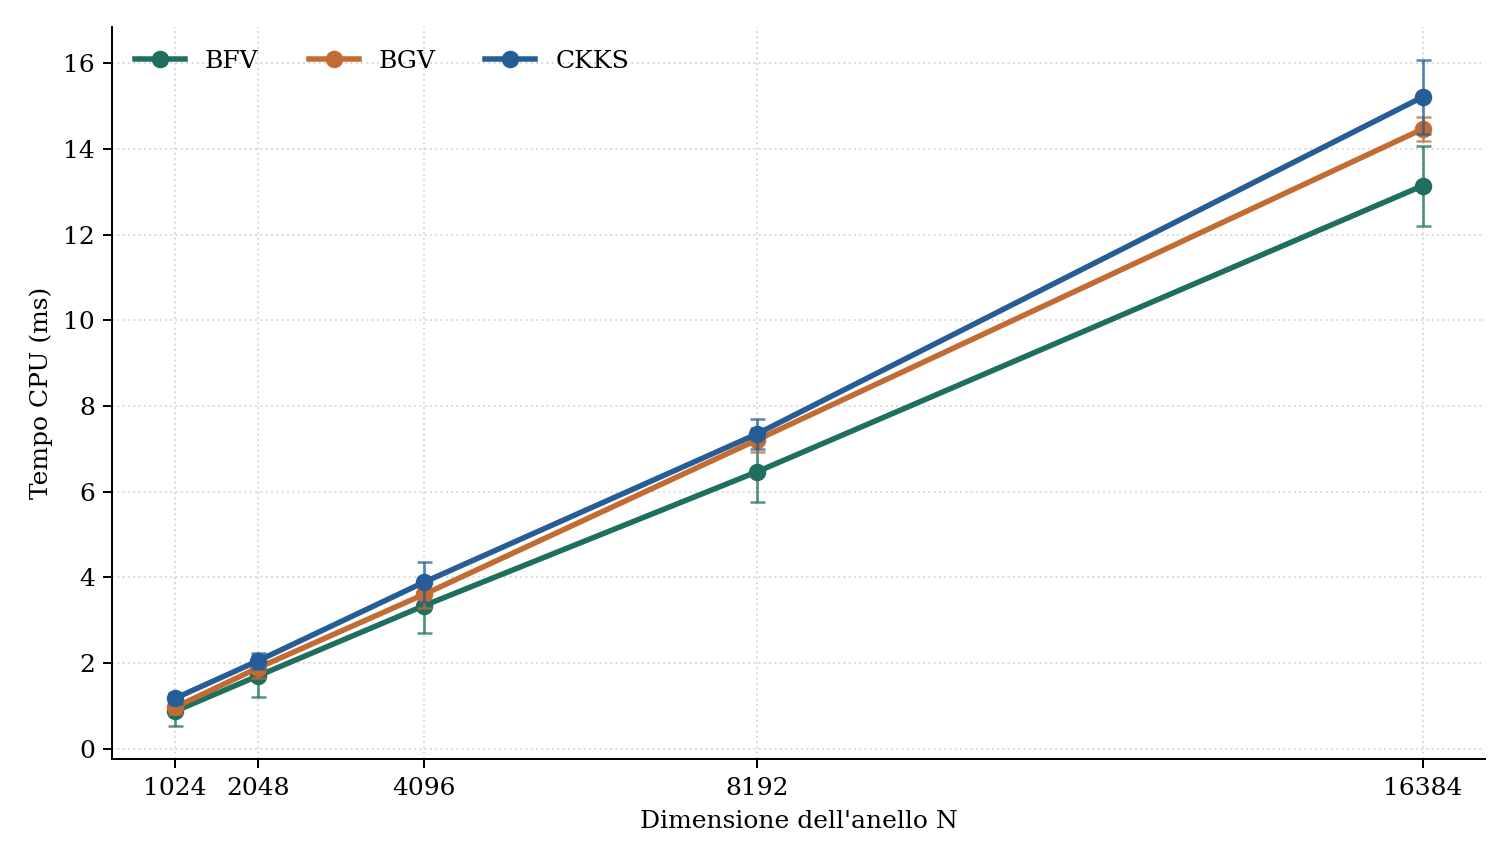
\includegraphics[width=0.64\textwidth]{figures/benchmark_encrypt.png}
\caption{Tempo di cifratura con profondit\`a 16.}
\label{fig:benchmark_encrypt}
\end{figure}

\begin{figure}[H]
\centering
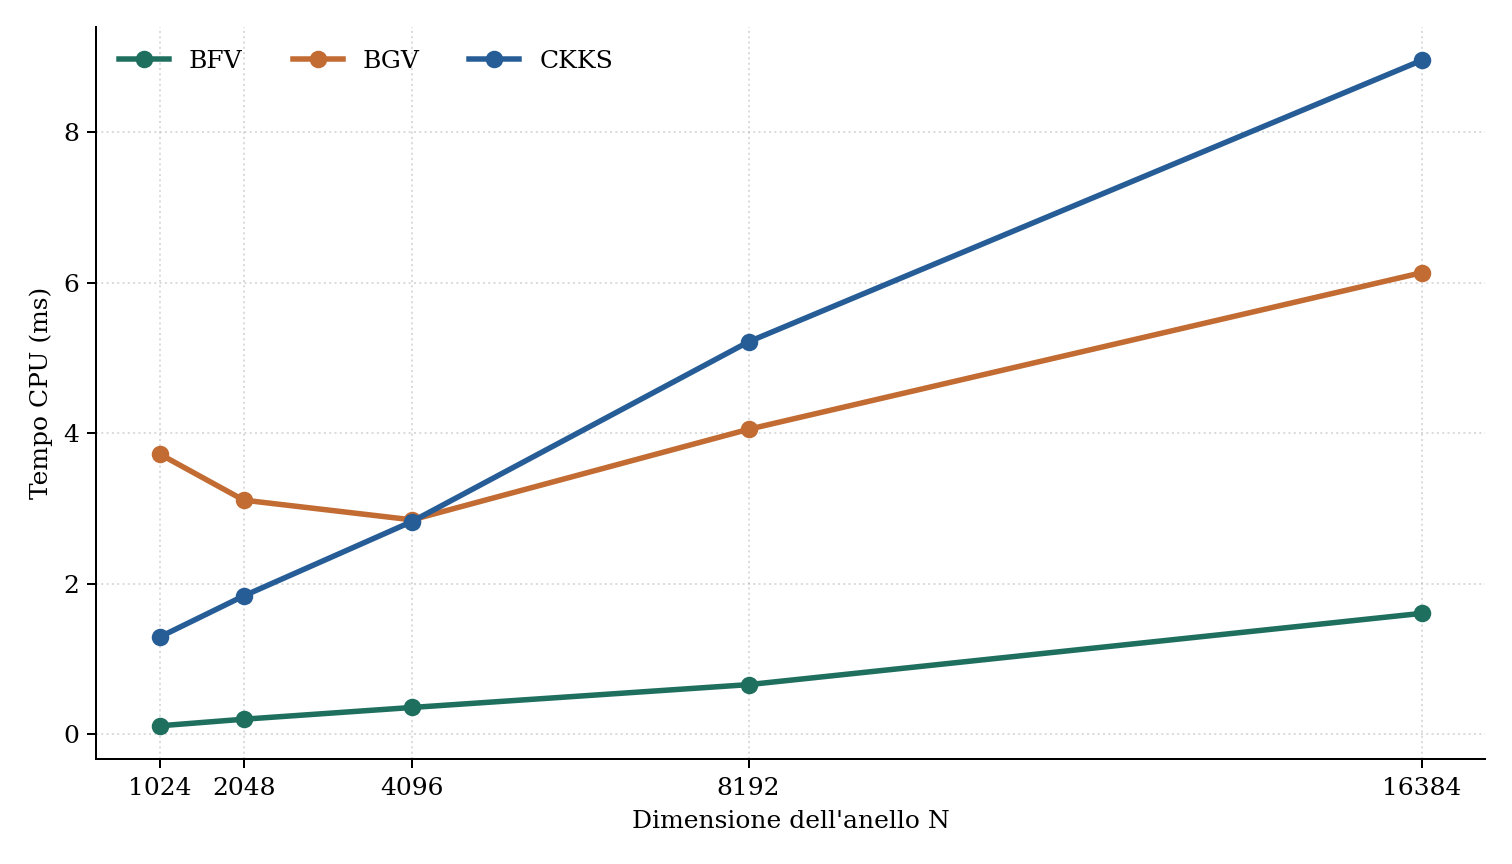
\includegraphics[width=0.64\textwidth]{figures/benchmark_decrypt.png}
\caption{Tempo di decifratura con profondit\`a 16.}
\label{fig:benchmark_decrypt}
\end{figure}

La cifratura cresce in modo abbastanza regolare con la ring dimension per tutti e tre gli schemi. Nel complesso, i tre andamenti restano piuttosto vicini: nessuno schema mostra un vantaggio netto e costante, e il grafico suggerisce soprattutto che il costo di \texttt{Encrypt} aumenta in modo simile al crescere di $N$.

La decifratura mostra invece differenze pi\`u nette. BFV resta chiaramente lo schema pi\`u rapido in tutto l'intervallo osservato. Tra gli altri due, CKKS tende a richiedere pi\`u tempo di BGV, soprattutto quando la ring dimension cresce. Il distacco principale, quindi, non \`e tra CKKS e BGV, ma tra questi due schemi e BFV.

Una dimensione maggiore offre anche pi\`u slot: BFV e BGV possono inserire $N$ interi, mentre CKKS inserisce $N/2$ valori complessi. Questo aumenta la quantit\`a di dati elaborabili in parallelo, ma rende anche pi\`u costose le singole operazioni.

\section{Somma e moltiplicazione}
Le Figure~\ref{fig:benchmark_add} e~\ref{fig:benchmark_mult} confrontano le due principali operazioni eseguite sui ciphertext.

\begin{figure}[H]
\centering
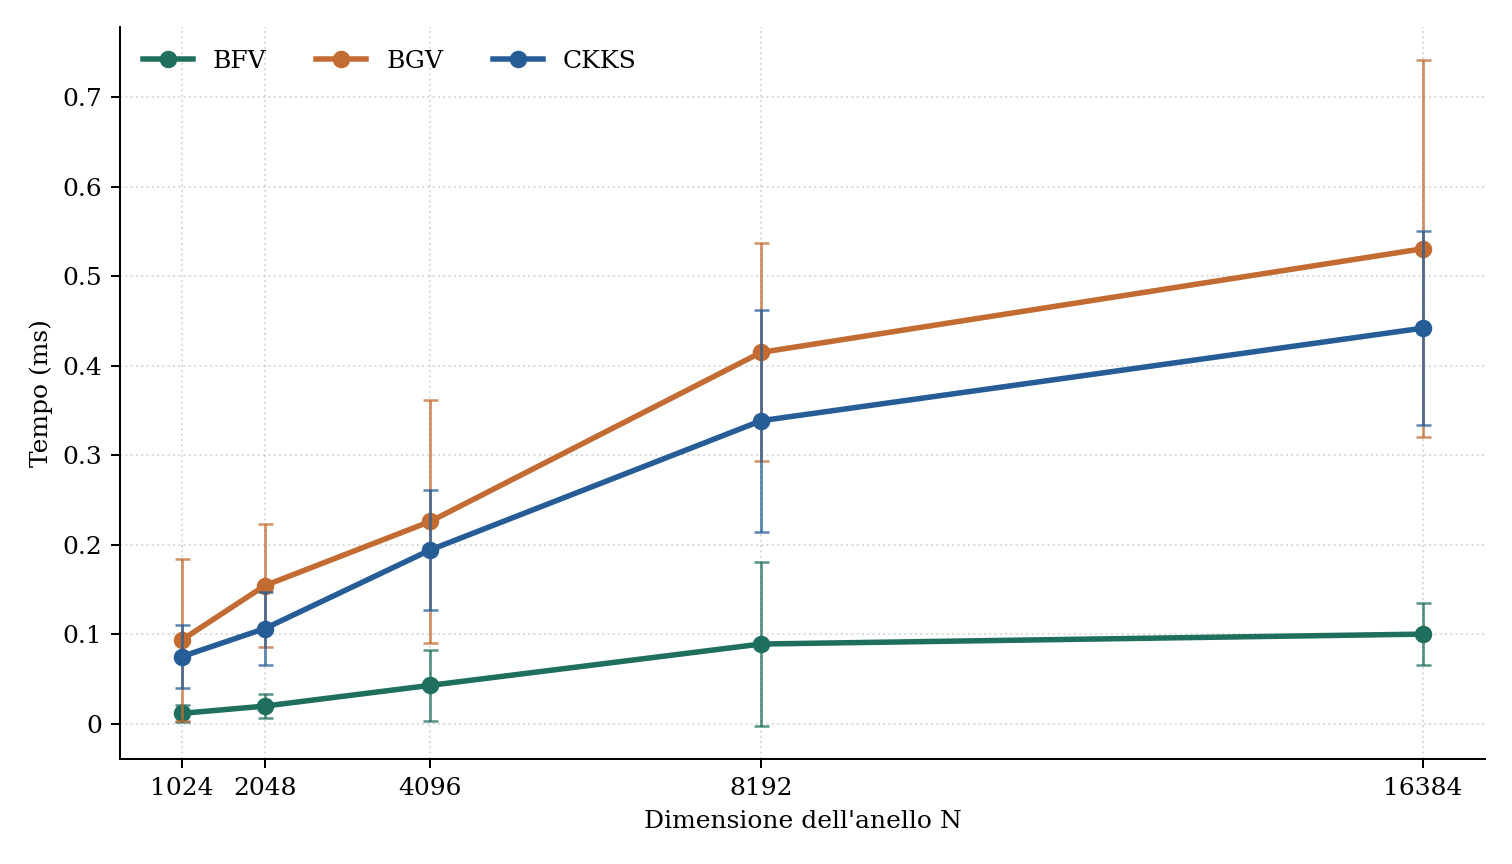
\includegraphics[width=0.64\textwidth]{figures/benchmark_add.png}
\caption{Tempo di una somma omomorfica con profondit\`a 16.}
\label{fig:benchmark_add}
\end{figure}

\begin{figure}[H]
\centering
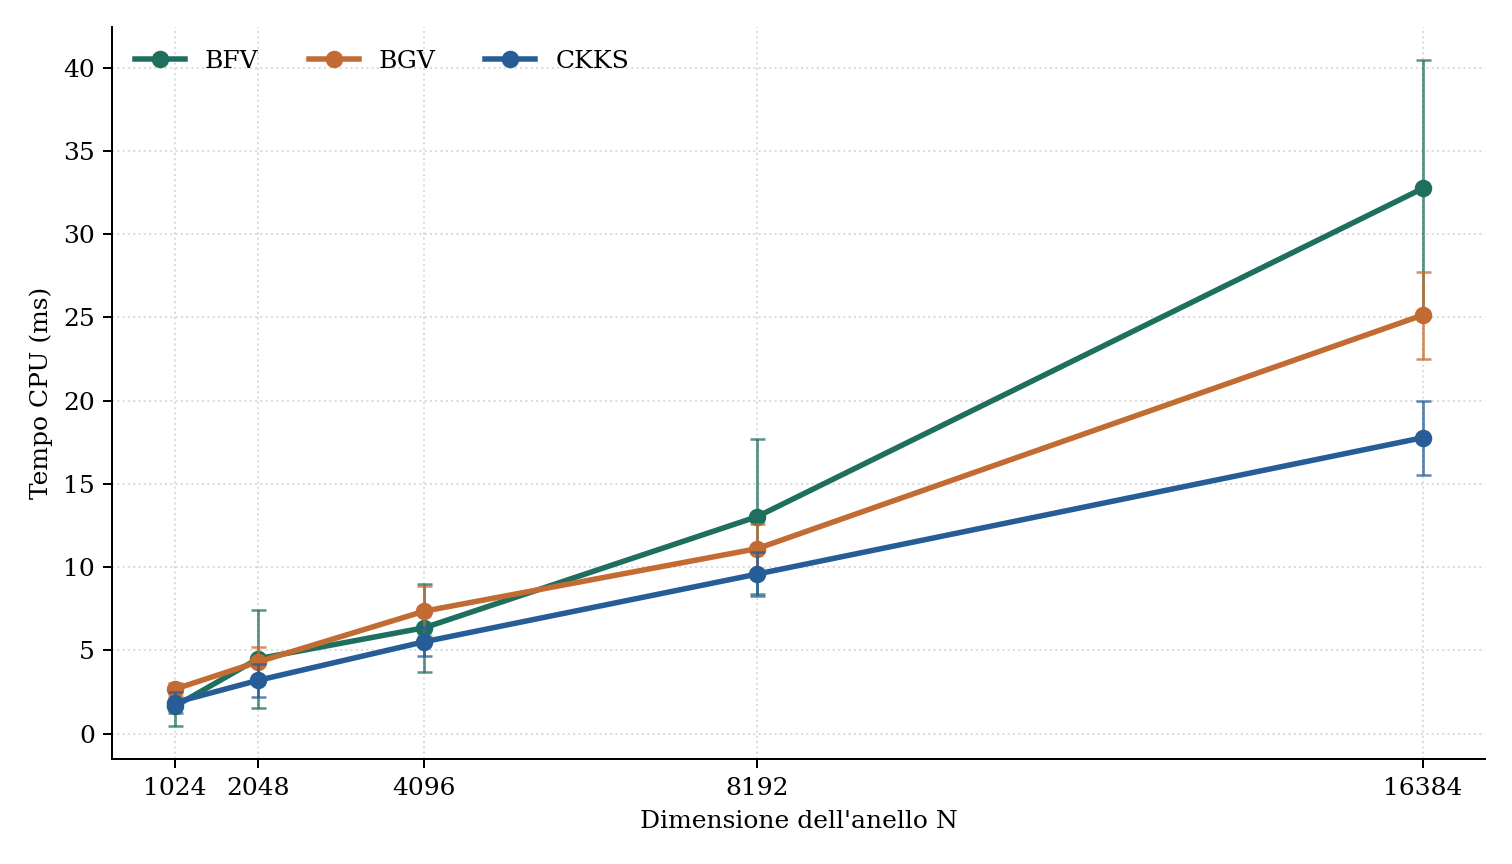
\includegraphics[width=0.64\textwidth]{figures/benchmark_mult.png}
\caption{Tempo di una moltiplicazione omomorfica con profondit\`a 16.}
\label{fig:benchmark_mult}
\end{figure}

La somma \`e chiaramente l'operazione pi\`u economica. I tre schemi restano tutti su valori molto bassi, con differenze contenute, anche se BGV tende a risultare un po' pi\`u pesante degli altri due. CKKS mostra l'andamento pi\`u leggero nel complesso, mentre BFV rimane vicino soprattutto nelle dimensioni intermedie e grandi.

La moltiplicazione cambia nettamente il quadro. Tutti gli schemi crescono con la ring dimension, ma BFV diventa molto pi\`u costoso di BGV e CKKS lungo quasi tutto l'intervallo osservato. Tra questi ultimi due, CKKS risulta in genere leggermente pi\`u rapido, mentre BGV gli resta vicino. Il dato principale che emerge dal grafico \`e quindi la distanza tra \texttt{EvalAdd} e \texttt{EvalMult}, e soprattutto il peso molto maggiore della moltiplicazione in BFV.

Le somme beneficiano del packing, che applica la stessa operazione a tutti gli slot. Quando invece il calcolo richiede controlli, prodotti tra valori o passaggi di machine learning, le moltiplicazioni diventano una parte importante della latenza.

\begin{table}[H]
\centering
\small
\begin{tabular}{lrrr}
\toprule
\textbf{Operazione, $N=4096$} & \textbf{BFV} & \textbf{BGV} & \textbf{CKKS} \\
\midrule
Cifratura & 5,496 ms & 3,906 ms & 3,846 ms \\
Somma & 0,158 ms & 0,232 ms & 0,085 ms \\
Moltiplicazione & 13,652 ms & 4,392 ms & 3,879 ms \\
Decifratura & 0,358 ms & 2,849 ms & 2,827 ms \\
\bottomrule
\end{tabular}
\caption{Tempi CPU con profondit\`a 16 e ring dimension 4096.}
\label{tab:benchmark_4096}
\end{table}

La Tabella~\ref{tab:benchmark_4096} mostra che una moltiplicazione costa molto pi\`u di una somma. Inoltre, le moltiplicazioni consumano livelli e richiedono evaluation keys. Il costo di una validazione omomorfica non dipende quindi solo dal numero di report, ma soprattutto dalla difficolta del circuito in cui essi saranno valutati.

\section{Memoria e interpretazione dei risultati}
La memoria registrata dalla suite non rappresenta il costo isolato del singolo ciphertext. Il processo mantiene contesto, chiavi e strutture create per il benchmark corrente. Inoltre, l'allocatore pu\`o conservare memoria tra operazioni. I valori devono quindi essere letti come impronta del processo e non come dimensione esatta di un oggetto.

La Figura~\ref{fig:benchmark_memory} mostra comunque la tendenza generale al crescere di $N$.

\begin{figure}[H]
\centering
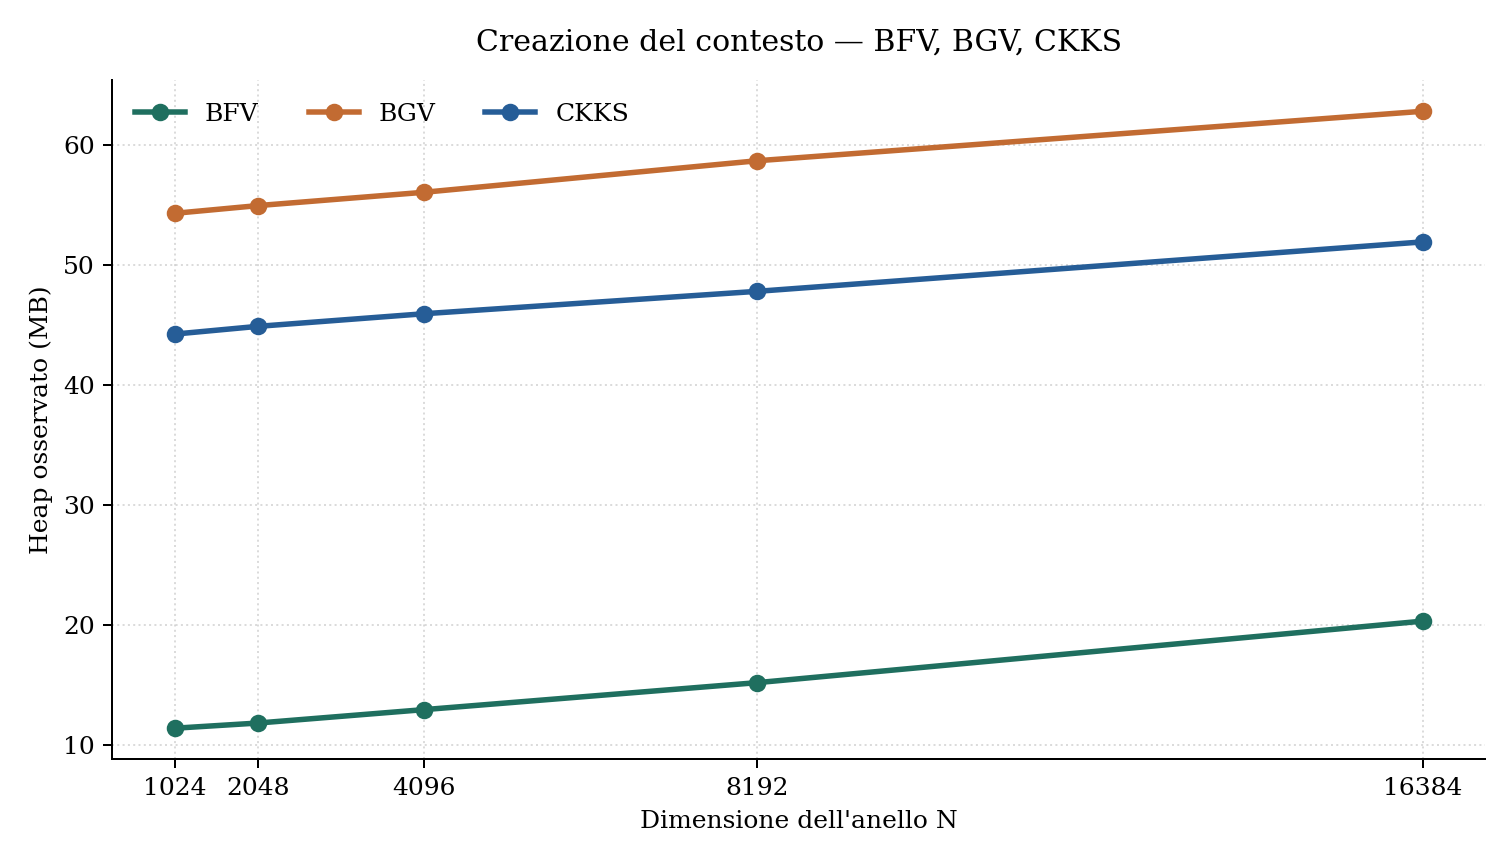
\includegraphics[width=0.64\textwidth]{figures/benchmark_memory.png}
\caption{Heap osservato durante la cifratura, con profondit\`a 16.}
\label{fig:benchmark_memory}
\end{figure}

BFV mostra nel processo di prova un livello di memoria molto inferiore rispetto a BGV e CKKS. I valori assoluti di BGV e CKKS includono memoria mantenuta dalla sequenza sperimentale e non devono essere interpretati come un confronto perfettamente isolato. La conclusione affidabile \`e pi\`u generale: contesti profondi, dimensioni maggiori ed evaluation keys possono richiedere gigabyte, rendendo la memoria un vincolo reale.

\section{Il costo particolare del bootstrapping}
CKKS include due benchmark aggiuntivi dedicati al bootstrapping. Il suo costo non dipende direttamente dal valore di profondit\`a usato, ma soprattutto dalla ring dimension. In pratica, aumentando $N$, anche il costo del bootstrapping cresce in modo evidente.

Questo rende il bootstrapping un'operazione molto pi\`u pesante delle somme e delle moltiplicazioni ordinarie. In calcoli poco profondi non \`e quindi conveniente, mentre diventa interessante soltanto quando serve proseguire un'elaborazione che altrimenti esaurirebbe i livelli disponibili.

Il confronto evidenzia una regola pratica: prima di ricorrere al bootstrapping conviene aumentare la profondit\`a, separare il calcolo in fasi o verificare se una configurazione leveled sia sufficiente.

\section{Scelta dello schema}
Se si vogliono usare numeri interi oppure aritmetica modulare, la scelta naturale \`e BFV o BGV. Tra questi due, BFV pu\`o andare bene quando il calcolo resta semplice, mentre BGV diventa in genere preferibile quando si usano operazioni pi\`u dispendiose della sola somma, in particolare le moltiplicazioni.

CKKS \`e invece la scelta adatta quando i dati non sono interi oppure quando si vogliono rappresentare numeri complessi. In questo caso bisogna accettare che il risultato sia approssimato e non esatto come negli schemi basati su interi.

\begin{table}[H]
\centering
\small
\begin{tabular}{p{2.3cm}p{3.2cm}p{3.2cm}p{3.2cm}}
\toprule
 & \textbf{BFV} & \textbf{BGV} & \textbf{CKKS} \\
\midrule
Dati & Interi & Interi & Reali o complessi \\
Risultato & Esatto modulo $p$ & Esatto modulo $p$ & Approssimato \\
Caso naturale & Conteggi e somme & Conteggi e controlli modulari & Statistica e machine learning \\
Attenzione & Overflow modulare & Overflow e profondit\`a & Precisione e rescaling \\
\bottomrule
\end{tabular}
\caption{Lettura applicativa dei tre schemi.}
\label{tab:scelta_schema}
\end{table}

\section{Limiti del benchmark}
I risultati sono stati raccolti su una sola macchina e in un ambiente WSL. Non sono presenti intervalli di confidenza tra esecuzioni indipendenti, misure energetiche o costi di rete. La memoria dipende dal comportamento dell'allocatore e dall'ordine dei test.

Il confronto usa parametri simili per rendere visibili le tendenze, ma gli schemi non offrono esattamente la stessa semantica. Infine, l'uso di \texttt{HEStd\_NotSet} impedisce di associare automaticamente ogni punto a uno specifico livello di sicurezza.

Questi limiti non annullano il valore dell'esperimento. I dati mostrano in modo chiaro che la ring dimension incide sul costo, che la somma \`e molto meno onerosa della moltiplicazione e che il bootstrapping \`e una fase eccezionalmente costosa. Sono proprio queste osservazioni a guidare le applicazioni dei capitoli successivi.

\section{Conclusioni}
I benchmark mostrano una tendenza chiara. Il packing permette di elaborare pi\`u valori in parallelo, ma dimensioni maggiori aumentano tempo e memoria.

Quando il sistema aggiunge moltiplicazioni, validazioni o training iterativo, il costo cambia sensibilmente. La profondit\`a e le evaluation keys diventano centrali; il bootstrapping deve essere usato solo quando necessario. I benchmark costituiscono quindi il collegamento tra le caratteristiche teoriche degli schemi e le scelte architetturali dei due casi di studio.

\chapter{Applicazioni di elaborazioni omomorfiche a scenari medicali}

\section{Introduzione}
In questo capitolo si considera un'applicazione concreta: l'uso della regressione lineare in uno scenario medico. L'idea di fondo \`e semplice. Pi\`u strutture sanitarie o pi\`u soggetti che raccolgono dati clinici vogliono contribuire alla costruzione di un modello statistico, ma senza rinunciare alla protezione delle informazioni trattate.

Nel caso concreto considerato, la regressione lineare viene usata per stimare il numero di giorni di permanenza in ospedale di un paziente a partire da et\`a, indice di comorbilit\`a di Charlson, numero di procedure precedenti, pressione sistolica e diastolica e indice di massa corporea. Il capitolo mostra come questo modello venga inserito in un'architettura i cui attori principali sono:
\begin{itemize}
  \item il \emph{setup authority}, che crea il contesto crittografico e genera le chiavi del sistema;
  \item il \emph{data provider}, che possiede i dati clinici originari;
  \item il \emph{computation server}, che esegue il training del modello o le valutazioni numeriche;
  \item il \emph{query actor}, che desidera interrogare il modello;
  \item il \emph{decryptor}, che pu\`o coincidere con un soggetto istituzionale, ad esempio il SSN, e che detiene la capacit\`a di decifrare i risultati.
\end{itemize}

La separazione tra computation server e decryptor \`e intenzionale. Le computazioni omomorfiche possono richiedere tempi elevati e possono quindi essere affidate anche a soggetti terzi specializzati, senza esporre in chiaro i dati sensibili o le query dei pazienti. Il decryptor resta invece il soggetto che possiede la chiave segreta e rende leggibile solo il risultato finale. A monte, il setup authority inizializza il sistema e distribuisce chiave pubblica, chiave segreta ed eventuali evaluation keys agli attori autorizzati.

Nel primo scenario il query actor invia query cifrate al computation server e riceve un risultato cifrato, poi decifrato dal decryptor. Nel secondo il computation server invia il polinomio cifrato al decryptor, mentre il query actor interroga in chiaro il servizio del soggetto fiduciario.

\section{Richiami sulla regressione lineare}
La regressione lineare serve a trovare una relazione semplice tra dati in ingresso e dato in uscita. In altre parole, si parte da esempi gi\`a osservati e si cerca una formula che descriva il loro andamento medio.

Il dataset contiene pi\`u osservazioni, una per ciascun paziente. Ogni osservazione comprende sei valori di ingresso: et\`a, indice di comorbilit\`a di Charlson, numero di procedure precedenti, pressione sistolica, pressione diastolica e indice di massa corporea. A questi sei valori corrisponde un unico valore da prevedere, cio\`e il numero di giorni di permanenza in ospedale.

Nel caso con pi\`u variabili in ingresso, il modello si scrive come
\begin{equation}
\hat{y} = w^T x + b = \sum_{j=1}^{6} w_j x_j + b,
\end{equation}
dove:
\begin{itemize}
  \item $w$ contiene i coefficienti del modello;
  \item $x$ contiene i sei valori di ingresso relativi al paziente;
  \item $b$ \`e il bias;
  \item $\hat{y}$ \`e il numero stimato di giorni di permanenza in ospedale.
\end{itemize}

La regressione adottata \`e lineare perch\'e tutte le variabili $x_j$ compaiono esclusivamente alla prima potenza: il modello non contiene termini quadratici, potenze superiori o interazioni tra feature. Questa scelta costituisce una semplificazione intenzionale. Variabili come la pressione sistolica e diastolica possono infatti avere una relazione pi\`u complessa e non lineare con la durata del ricovero; in un'applicazione clinica completa si potrebbero quindi considerare trasformazioni delle feature o modelli differenti. Nel presente caso si mantiene invece una funzione affine di primo grado, poich\'e lo scopo principale \`e dimostrare in modo semplice e leggibile l'applicazione delle tecniche omomorfiche.

\subsection{Funzione di costo}
Per capire se la retta trovata \`e buona oppure no, bisogna confrontare le previsioni del modello con i valori reali. Durante l'ottimizzazione si considera la met\`a dell'errore quadratico medio:
\begin{equation}
J(w,b) = \frac{1}{2n}\sum_{i=1}^{n}(\hat{y}_i - y_i)^2.
\end{equation}
Il fattore $1/2$ semplifica il calcolo del gradiente e non cambia i valori di $w$ e $b$ che minimizzano la funzione. La MSE completa, pari a $2J(w,b)$, viene usata per monitorare l'andamento del training. Se $J(w,b)$ \`e piccolo, il modello rappresenta bene le osservazioni disponibili.

\subsection{Determinazione dei coefficienti}
I coefficienti non vengono ricavati calcolando direttamente l'inversa di una matrice. Il modello usa invece la \emph{discesa del gradiente} (\emph{gradient descent}), un procedimento iterativo che parte da coefficienti iniziali molto semplici e li corregge poco alla volta nella direzione che riduce la funzione di costo.

Il training parte da pesi e bias nulli e, per un numero prefissato di epoche, calcola la previsione, misura l'errore e aggiorna i coefficienti usando un learning rate $\eta$.

In forma compatta, la previsione del modello \`e
\begin{equation}
\hat{y} = Xw + b\mathbf{1}_n,
\end{equation}
 dove $\mathbf{1}_n$ \`e un vettore di $n$ elementi uguali a uno e indica che lo stesso bias viene aggiunto alla previsione di ogni paziente.
Successivamente si calcola il vettore degli errori:
\begin{equation}
E = \hat{y} - y.
\end{equation}
Se una previsione \`e troppo alta rispetto al valore reale, l'errore sar\`a positivo; se invece \`e troppo bassa, l'errore sar\`a negativo.

Una volta ottenuto l'errore, il modello aggiorna i pesi tramite
\begin{equation}
w \leftarrow w - \eta \frac{1}{n} X^T E
\end{equation}
e aggiorna il bias tramite
\begin{equation}
b \leftarrow b - \eta \cdot \frac{1}{n}\sum_{i=1}^{n} E_i.
\end{equation}

Se il modello sbaglia sistematicamente in una direzione, i coefficienti vengono spostati gradualmente nella direzione opposta. La MSE viene calcolata a ogni epoca per verificare il miglioramento.

\subsection{Interpretazione in ambito medico}
Nel caso considerato, il modello assume la forma
\begin{equation}
\hat{y}=w_1\,\text{age}+w_2\,\text{cci}
+w_3\,\text{num\_procedures}+w_4\,\text{systolic}
+w_5\,\text{diastolic}+w_6\,\text{bmi}+b,
\end{equation}
dove $\hat{y}$ \`e la permanenza stimata in ospedale, espressa in giorni. I coefficienti descrivono il contributo delle singole feature:
\begin{itemize}
  \item $w_1$ \`e associato all'et\`a del paziente, compresa nell'intervallo $[0,100]$ anni;
  \item $w_2$ \`e associato al Charlson Comorbidity Index, compreso nell'intervallo $[0,37]$;
  \item $w_3$ \`e associato al numero di procedure o interventi precedenti, compreso nell'intervallo $[0,20]$;
  \item $w_4$ \`e associato alla pressione sistolica, compresa nell'intervallo $[80,200]$ mmHg;
  \item $w_5$ \`e associato alla pressione diastolica, compresa nell'intervallo $[50,120]$ mmHg;
  \item $w_6$ \`e associato all'indice di massa corporea, compreso indicativamente nell'intervallo $[15,40]$;
  \item $b$ rappresenta il bias del modello.
\end{itemize}

Questi intervalli descrivono i valori attesi delle variabili di ingresso, non i possibili valori dei coefficienti appresi. Inoltre, i coefficienti esprimono associazioni apprese dal dataset e non relazioni causali.

\section{Regressione lineare ed elaborazione omomorfica}
Una volta costruito il modello, il passaggio successivo consiste nel capire come usarlo nei due scenari considerati. La regressione lineare si presta bene a questo contesto perch\'e, una volta noti i coefficienti, la previsione si ottiene con un calcolo molto semplice:
\begin{equation}
\hat{y} = w^T x + b = \sum_{j=1}^{d} w_j x_j + b.
\end{equation}
In sostanza, bisogna fare prodotti e somme. Questo rende il modello adatto a un uso pratico anche in un'architettura protetta, perch\'e la fase di inferenza non richiede logiche troppo complicate.

L'implementazione in FHE usa lo schema CKKS. Questa scelta \`e utile perch\'e consente di rappresentare ed elaborare anche valori non interi, caratteristica importante in regressione lineare quando coefficienti, medie o risultati intermedi non sono interi. Inoltre, nell'implementazione si ricorre al \emph{bootstrapping} per riazzerare la profondit\`a moltiplicativa del ciphertext, poich\'e durante la regressione lineare, in particolare nelle fasi iterative di calcolo, si accumulano molte moltiplicazioni omomorfiche. CKKS introduce approssimazioni numeriche e quindi piccoli errori di arrotondamento, ma nel contesto considerato tali differenze sono trascurabili ai fini del risultato finale.

Nel calcolo in chiaro si pu\`o pensare a $x$, $w$ ed $y$ come a vettori e matrici ordinarie. In FHE, invece, questi dati devono essere inseriti negli slot di un ciphertext. Per questo motivo l'implementazione non lavora direttamente con la matrice nella sua forma pi\`u intuitiva, ma la riorganizza in blocchi che possano essere sommati e ruotati in modo efficiente.

Nel presente contesto si pu\`o scomporre il problema in due fasi:
\begin{enumerate}
  \item \textbf{training del modello}: il computation server riceve i dati dai provider e costruisce i coefficienti della regressione;
  \item \textbf{inferenza o query}: un attore interroga il modello per ottenere una previsione su un nuovo input.
\end{enumerate}

Il punto interessante \`e che nei due scenari cambia soprattutto la fase di query. Il modello matematico resta lo stesso, ma cambia chi vede i dati in chiaro, chi esegue la valutazione finale e chi possiede le chiavi necessarie per decifrare.

\section{Scenario 1: query cifrata al computation server}
Nel primo scenario, il data provider invia i dati al computation server, che esegue la regressione lineare e costruisce il polinomio del modello. Successivamente, il query actor non invia un input in chiaro, ma una query cifrata. Il computation server valuta il modello sul dato cifrato e restituisce un risultato anch'esso cifrato. Infine, il query actor si rivolge a un servizio di decrypt, che pu\`o essere incarnato dal SSN, per ottenere il valore in chiaro.

\subsection{Schema logico}
Lo schema pu\`o essere rappresentato come segue, assumendo che il setup authority distribuisca preventivamente le chiavi ai vari attori autorizzati:
\begin{align}
&\text{Data Provider}_i \longrightarrow \text{Computation Server}: \mathsf{Enc}_{pk}(\text{record di training}_i), \\
&\text{Computation Server}: \text{training su dati cifrati e costruzione di } \mathsf{Enc}_{pk}(w,b), \\
&\text{Query Actor} \longrightarrow \text{Computation Server}: \mathsf{Enc}_{pk}(x_q), \\
&\text{Computation Server}: \text{valutazione del modello su } \mathsf{Enc}_{pk}(x_q), \\
&\text{Computation Server} \longrightarrow \text{Query Actor}: \mathsf{Enc}_{pk}(w^T x_q + b), \\
&\text{Query Actor} \longrightarrow \text{Decryptor/SSN}: \mathsf{Enc}_{pk}(w^T x_q + b), \\
&\text{Decryptor/SSN}: \mathsf{Dec}_{sk}\big(\mathsf{Enc}_{pk}(w^T x_q + b)\big), \\
&\text{Decryptor/SSN} \longrightarrow \text{Query Actor}: w^T x_q + b.
\end{align}

Il computation server addestra il modello e valuta il polinomio su query cifrate; il query actor vede il risultato in chiaro solo dopo l'intervento del decryptor.

\begin{figure}[H]
\centering
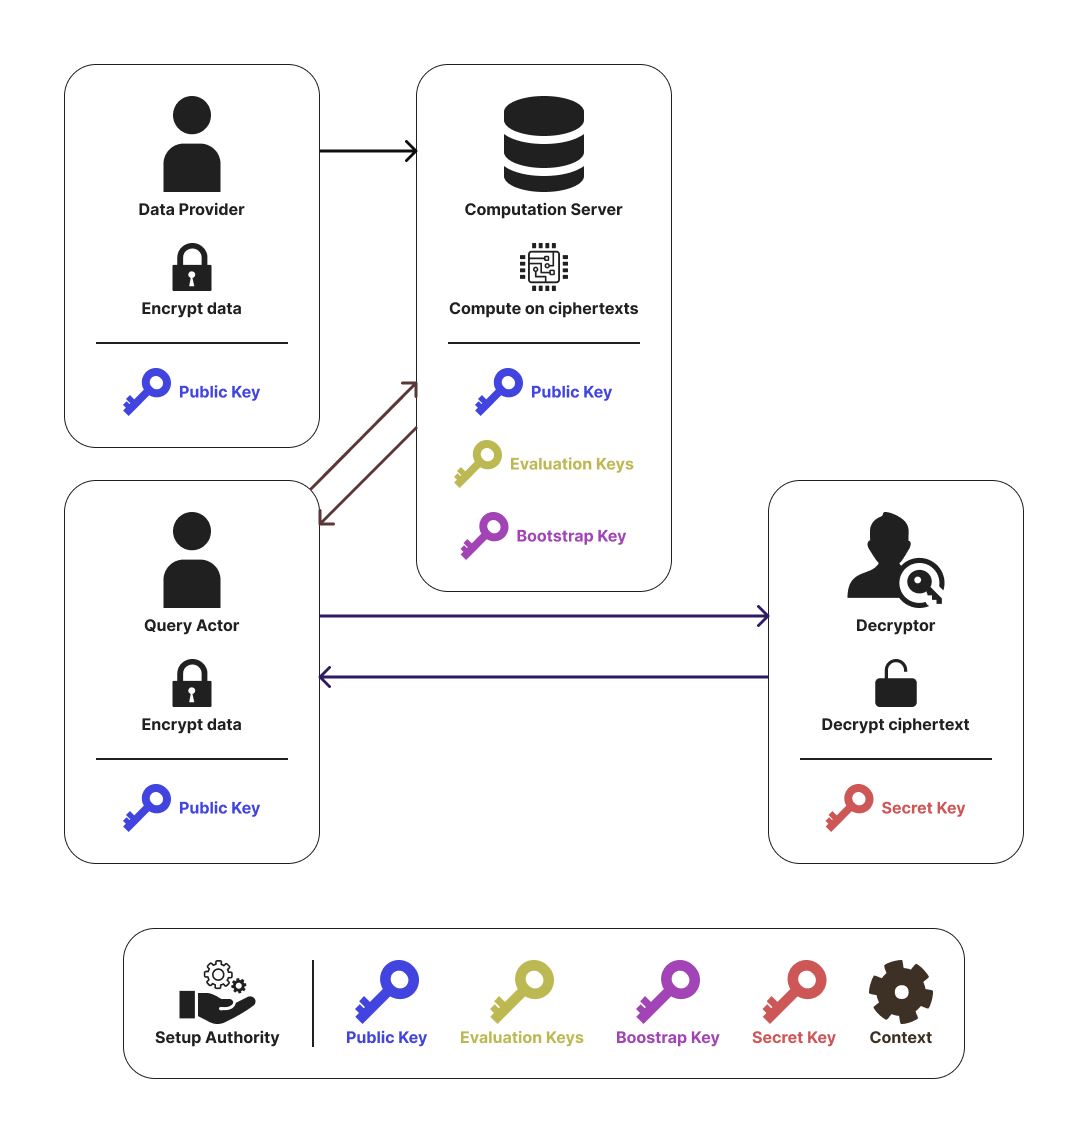
\includegraphics[width=0.95\textwidth]{figures/linear_regression_1.png}
\caption{Schema dello scenario 1.}
\label{fig:linear_regression_1}
\end{figure}

\subsection{Distribuzione delle chiavi}
In questo scenario si assume tipicamente la seguente ripartizione:
\begin{itemize}
  \item il \textbf{setup authority} genera il contesto crittografico, la chiave pubblica $pk$, la chiave segreta $sk$ ed eventuali evaluation keys, poi distribuisce tale materiale ai ruoli autorizzati;
  \item i \textbf{data provider} inviano al computation server soltanto dati cifrati con $pk$;
  \item il \textbf{computation server} conosce la chiave pubblica $pk$ e le eventuali evaluation keys necessarie alle operazioni omomorfiche;
  \item il \textbf{query actor} possiede o riceve la chiave pubblica $pk$ per cifrare le query;
  \item il \textbf{decryptor/SSN} possiede la chiave segreta $sk$;
\end{itemize}

La propriet\`a essenziale \`e che il computation server non dispone di $sk$, dunque non pu\`o vedere il contenuto delle query finali n\'e dei risultati cifrati che produce.

Lo scenario protegge la query e separa chi calcola da chi decifra. Richiede per\`o cifratura lato utente, gestione delle evaluation keys e l'intervento del decryptor, con maggiore complessit\`a e latenza.

\section{Scenario 2: il polinomio cifrato viene trasferito al decryptor}
Nel secondo scenario, il data provider invia i dati al computation server, che esegue il training del modello. Una volta ottenuti i coefficienti della regressione, il computation server cifra il polinomio e lo trasferisce direttamente al decryptor, ad esempio il SSN. Da quel momento, il query actor non interagisce pi\`u con il computation server per la fase di inferenza, ma invia le proprie query in chiaro al soggetto fiduciario.

\subsection{Schema logico}
Lo schema pu\`o essere espresso come segue, assumendo che il setup authority distribuisca preventivamente le chiavi ai vari attori autorizzati:
\begin{align}
&\text{Data Provider}_i \longrightarrow \text{Computation Server}: \mathsf{Enc}_{pk}(\text{record di training}_i), \\
&\text{Computation Server}: \text{training su dati cifrati e costruzione di } \mathsf{Enc}_{pk}(w,b), \\
&\text{Computation Server} \longrightarrow \text{Decryptor/SSN}: \mathsf{Enc}_{pk}(w,b), \\
&\text{Decryptor/SSN}: \mathsf{Dec}_{sk}\big(\mathsf{Enc}_{pk}(w,b)\big), \\
&\text{Query Actor} \longrightarrow \text{Decryptor/SSN}: x_q \text{ in chiaro}, \\
&\text{Decryptor/SSN} \longrightarrow \text{Query Actor}: w^T x_q + b.
\end{align}

Il query actor beneficia di un'interfaccia pi\`u semplice: non cifra nulla, ma si appoggia a un'entit\`a trusted che custodisce il modello e produce le risposte.

\begin{figure}[H]
\centering
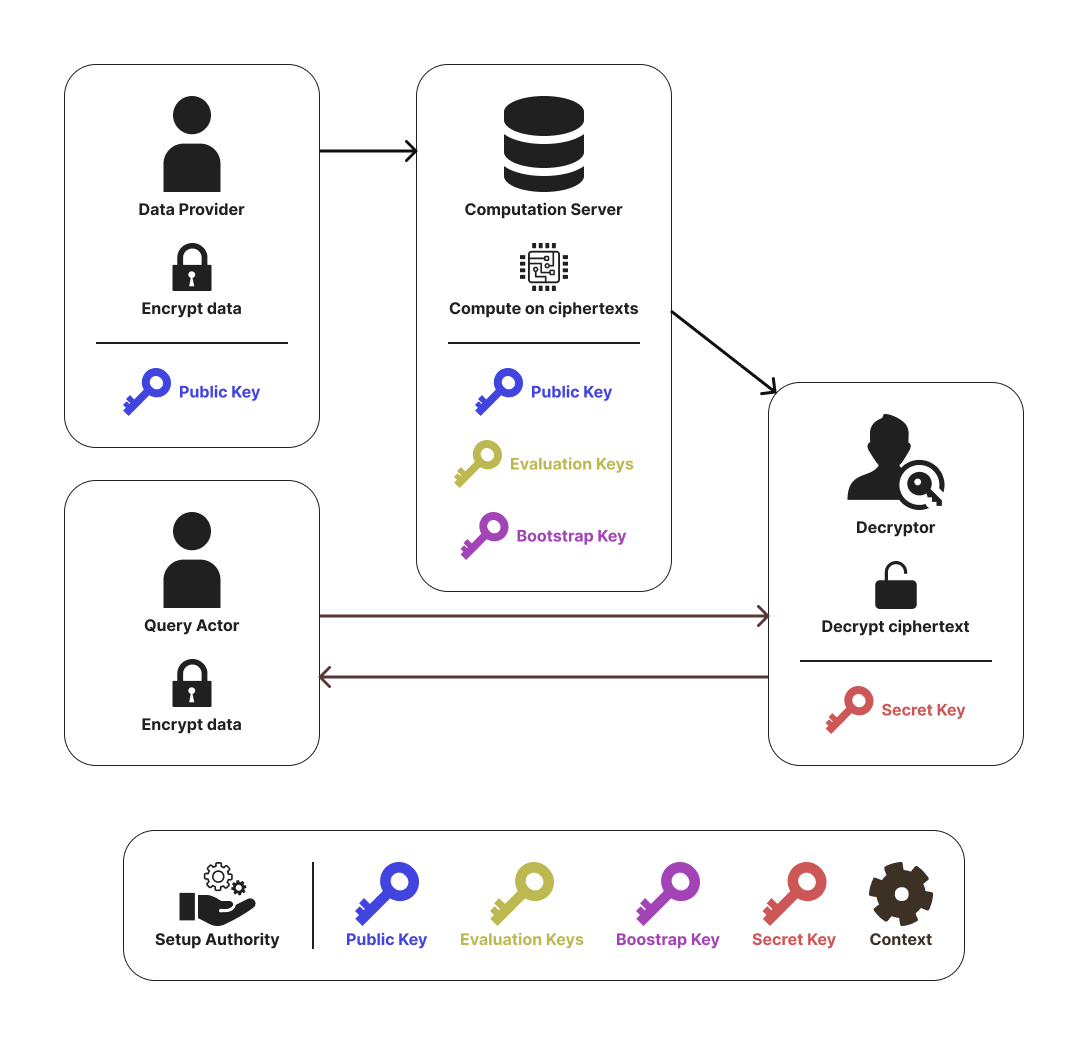
\includegraphics[width=0.95\textwidth]{figures/linear_regression_2.png}
\caption{Schema dello scenario 2.}
\label{fig:linear_regression_2}
\end{figure}

\subsection{Distribuzione delle chiavi}
La distribuzione delle chiavi \`e pi\`u centralizzata:
\begin{itemize}
  \item il \textbf{setup authority} genera il contesto crittografico, la chiave pubblica $pk$, la chiave segreta $sk$ ed eventuali evaluation keys, poi le distribuisce agli attori autorizzati;
  \item i \textbf{data provider} inviano al computation server soltanto dati cifrati con $pk$;
  \item il \textbf{computation server} conosce la chiave pubblica $pk$ e le eventuali evaluation keys necessarie alle operazioni omomorfiche;
  \item il \textbf{query actor} non ha bisogno di utilizzare direttamente chiavi crittografiche nella fase di interrogazione;
  \item il \textbf{decryptor/SSN} possiede la chiave segreta $sk$;
\end{itemize}

Questa architettura \`e coerente con contesti in cui il decryptor rappresenta un ente istituzionale gi\`a riconosciuto come fiduciario, in grado di custodire chiavi, modelli e risultati.

Lo scenario semplifica l'interrogazione e riduce la latenza, ma espone l'input al decryptor e concentra informazioni e fiducia presso tale ente. \`E quindi adatto quando la fiducia nel soggetto istituzionale \`e alta.

\section{Confronto tra le due architetture}
Le due architetture risolvono lo stesso problema, ma ottimizzano aspetti diversi. Una sintesi comparativa pu\`o essere espressa nella Tabella~\ref{tab:confronto_scenari}.

\begin{table}[h]
\centering
\begin{tabular}{|p{3.3cm}|p{5.2cm}|p{5.2cm}|}
\hline
\textbf{Aspetto} & \textbf{Scenario 1} & \textbf{Scenario 2} \\
\hline
Protezione delle query & Alta: il computation server riceve query cifrate & Pi\`u bassa: il query actor invia la query in chiaro al decryptor/SSN \\
\hline
Ruolo del computation server & Addestra il modello e valuta query cifrate & Addestra il modello e invia il polinomio cifrato al decryptor \\
\hline
Ruolo del decryptor & Decifra il risultato finale & Custodisce il modello e risponde alle query \\
\hline
Chiave segreta & Presso il decryptor/SSN & Presso il decryptor/SSN \\
\hline
Chiave pubblica & Usata da query actor e computation server & Usata da data provider e computation server \\
\hline
Complessit\`a per l'utente finale & Maggiore: deve cifrare la query & Minore: usa un'interfaccia in chiaro \\
\hline
Latenza complessiva & Pi\`u elevata & Pi\`u contenuta, ma con costo di inferenza a carico del decryptor/SSN \\
\hline
\end{tabular}
\caption{Confronto tra i due scenari di impiego della regressione lineare in ambito omomorfico-medicale.}
\label{tab:confronto_scenari}
\end{table}

Da questa tabella emerge un trade-off classico. Se si vuole proteggere fortemente la riservatezza dell'input di inferenza, lo scenario 1 \`e generalmente preferibile. Se invece si desidera un servizio pi\`u semplice, controllato da un ente sanitario centrale e pi\`u immediato da usare, lo scenario 2 pu\`o risultare pi\`u naturale. Va per\`o ricordato che, nello scenario 2, il training resta a carico del computation server mentre l'inferenza viene eseguita dal decryptor, cio\`e dal SSN: anche questa fase ha quindi un costo computazionale e operativo che deve essere sostenuto dall'attore ultimo invece del server computazionale che però essendo in chiaro risultat molto meno dispendioso del eseguire una decrifrazione.

\section{Esempio applicativo: stima dei giorni di ricovero}
Il dataset sanitario contiene, per ogni osservazione, le sei caratteristiche del paziente e il numero di giorni di permanenza in ospedale da apprendere. Alcune osservazioni sono:
\begin{center}
\begin{tabular}{|c|c|c|c|c|c|c|}
\hline
\textbf{Et\`a} & \textbf{CCI} & \textbf{Proc.} & \textbf{Sist.} &
\textbf{Diast.} & \textbf{BMI} & \textbf{Giorni} \\
\hline
37 & 2 & 12 & 148 & 106 & 22.5 & 4 \\
77 & 1 & 7 & 105 & 106 & 38.0 & 3 \\
83 & 2 & 17 & 82 & 64 & 29.2 & 5 \\
\hline
\end{tabular}
\end{center}

Il modello deve trovare i sei pesi e il bias che minimizzano l'errore tra i giorni stimati e quelli presenti nell'ultima colonna.

\subsection{Come parte il training}
Il training parte da coefficienti iniziali nulli:
\begin{equation}
w_1 = \cdots = w_6 = 0,
\qquad
b = 0.
\end{equation}

Con questa scelta, la previsione iniziale per ogni paziente \`e zero. Il computation server confronta tali previsioni con i giorni di permanenza osservati e usa gli errori per correggere pesi e bias. Il procedimento viene ripetuto epoca dopo epoca: i parametri non sono ottenuti in un singolo passaggio, ma attraverso un miglioramento progressivo del modello.

\subsection{Quale modello viene recuperato}
Il generatore costruisce una durata attesa a partire dalle caratteristiche del paziente. Et\`a, CCI e numero di procedure forniscono un contributo di base; valori pressori o BMI esterni agli intervalli considerati normali aggiungono un ulteriore contributo.

Il dataset non segue quindi una relazione lineare esatta. La regressione apprende una funzione affine che approssima l'andamento complessivo:
\begin{equation}
\widehat{\text{days\_in\_hospital}}=w^Tx+b.
\end{equation}
L'uscita va interpretata come una stima della permanenza e non come un valore clinico certo.

\subsection{Verifica su un nuovo dato}
Una query contiene le sei caratteristiche di un nuovo paziente, per esempio:
\begin{equation}
x_q=(50,4,20,128,96,26.7).
\end{equation}
Il modello calcola $\hat{y}=w^Tx_q+b$ e restituisce il numero stimato di giorni di permanenza in ospedale. Una volta ottenuti i coefficienti, la query richiede soltanto prodotti e somme e si presta quindi alla valutazione omomorfica.

\subsection{Lettura dell'esempio nei due scenari}
Nello \textbf{scenario 1}, il query actor cifra il vettore clinico $x_q$ e lo invia al computation server. Il server applica il modello al dato cifrato e produce
\begin{equation}
\mathsf{Enc}_{pk}(w^Tx_q+b),
\end{equation}
cio\`e la stima cifrata dei giorni di ricovero. Il risultato viene poi decifrato dal SSN.

Nello \textbf{scenario 2}, il computation server ha gi\`a trasmesso il polinomio cifrato al decryptor. Il SSN custodisce i coefficienti e riceve in chiaro il vettore clinico del paziente, sul quale calcola $w^Tx_q+b$. Il valore matematico finale \`e lo stesso; cambia il punto del sistema in cui i dati del paziente vengono esposti in chiaro.

\section{Aspetti operativi e limiti}
La cifratura omomorfica consente di analizzare dati distribuiti tra strutture sanitarie senza condividerli in forma leggibile. La semplicit\`a della regressione lineare la rende adatta a progetti pilota nei quali la trasparenza del modello \`e importante.

Restano limiti concreti: CKKS introduce piccole approssimazioni numeriche, il costo computazionale supera quello dell'elaborazione in chiaro e occorre gestire chiavi, audit, responsabilit\`a e validazione clinica.

\section{Conclusioni}
La regressione lineare rappresenta un caso di studio efficace per mostrare come la cifratura omomorfica possa essere applicata a scenari medicali concreti. Il computation server costruisce un polinomio di primo grado, o pi\`u in generale una funzione affine multivariata, a partire da dati clinici raccolti dai data provider. Successivamente tale modello pu\`o essere interrogato secondo architetture differenti, che riflettono scelte diverse in termini di privacy, fiducia e semplicit\`a operativa.

Lo scenario 1 privilegia la protezione della query e riduce l'esposizione del dato di input al computation server, ma richiede una pipeline pi\`u articolata. Lo scenario 2, invece, centralizza la fiducia nel decryptor, semplifica l'interrogazione e pu\`o adattarsi bene a una governance sanitaria istituzionale, pur esponendo in chiaro la query al soggetto fiduciario.

\chapter{Protocollo di aggregazione simil prio3 utilizzando tecniche omomorfiche}

\section{Introduzione}
Prio3 VDAF \`e, in modo molto semplice, un protocollo pensato per raccogliere dati da pi\`u client e calcolarne un risultato aggregato senza esporre il contributo individuale di ciascuno \cite{prio}. L'idea generale \`e che ogni client non invii direttamente il proprio valore in chiaro a un unico soggetto, ma produca una rappresentazione adatta a essere elaborata da pi\`u attori del protocollo. In questo modo, il sistema finale pu\`o recuperare il risultato complessivo senza ricostruire facilmente il dato del singolo partecipante.

L'obiettivo di questo capitolo \`e allora il seguente: replicare in ambiente FHE la forma generale di un protocollo di aggregazione ispirato a Prio3, mantenendo l'idea di fondo di raccolta privata e di validazione dei report, ma semplificando l'architettura. La costruzione che introduciamo, chiamata \texttt{fhe-vdaf}, usa lo schema omomorfico BGV: i report vengono cifrati dai client, inviati a un unico aggregatore, validati sotto cifratura e poi sommati, in modo che l'attore finale possa apprendere soltanto il risultato aggregato.

La scelta di BGV non \`e casuale. In questo contesto i report sono valori interi e tutta la logica di validazione viene espressa tramite aritmetica modulare. BGV \`e quindi naturale perch\'e lavora direttamente su interi modulo $p$. Questo significa che somme e moltiplicazioni avvengono nello stesso ambiente algebrico in cui vogliamo controllare i report, compreso il comportamento di overflow, che viene assorbito in modo coerente dalla riduzione modulo $p$.

\section{Idea generale di \texttt{fhe-vdaf}}
La struttura di \texttt{fhe-vdaf} pu\`o essere descritta in modo molto semplice:
\begin{enumerate}
  \item il client vuole inviare un valore numerico;
  \item lo converte in una rappresentazione binaria a slot;
  \item cifra tale rappresentazione con la chiave pubblica del sistema;
  \item invia il ciphertext all'aggregatore;
  \item l'aggregatore valida omomorficamente il report;
  \item se il report \`e valido, lo aggiunge alla somma aggregata;
  \item il collector finale decifra solo il totale.
\end{enumerate}

In pratica, tutti i report cifrati arrivano allo stesso aggregatore. La crittografia di base resta la stessa, ma cambia il modo in cui il sistema distribuisce i compiti e la fiducia tra gli attori.

\section{Ruoli architetturali e gestione delle chiavi}

\begin{figure}[H]
\centering
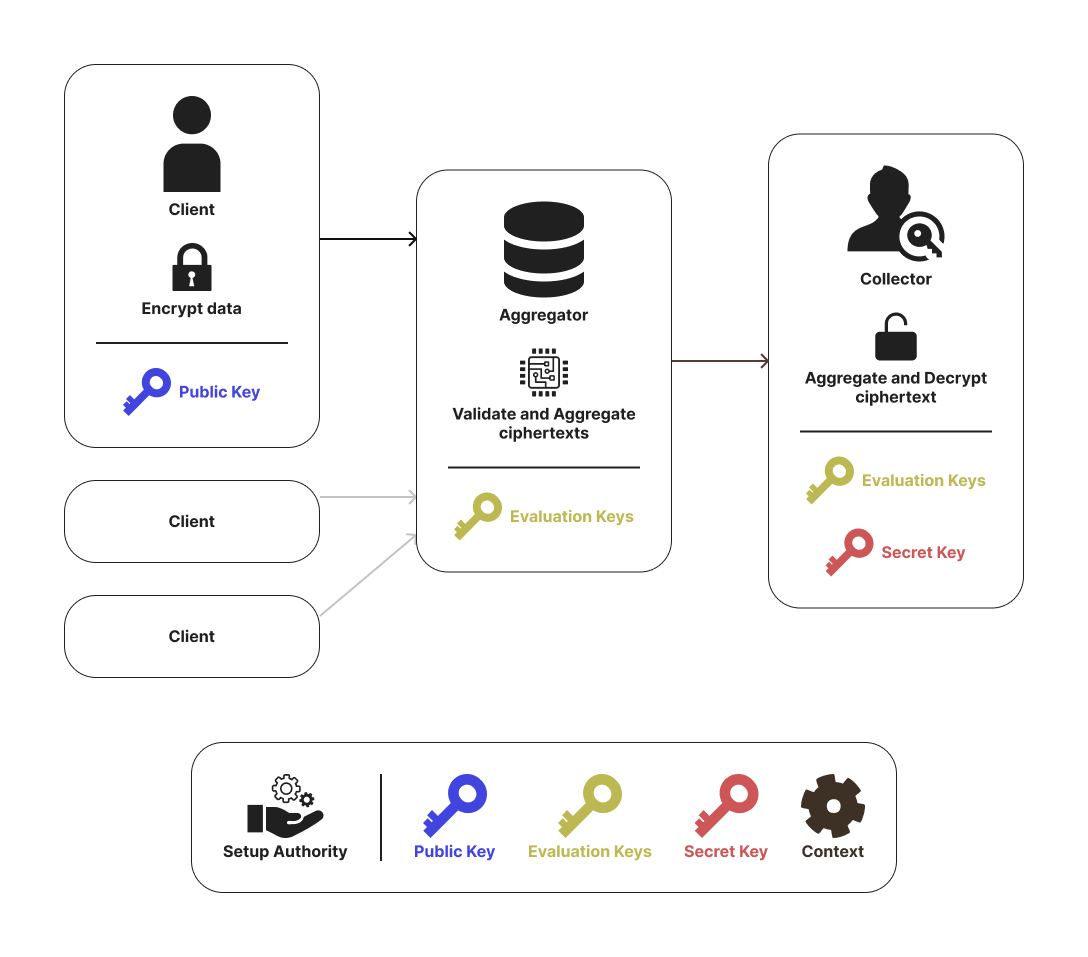
\includegraphics[width=0.95\textwidth]{figures/vdaf_0.png}
\caption{Schema di fhe-vdaf.}
\label{fig:vdaf_0}
\end{figure}

\subsection{Attori del sistema}
Nel caso di \texttt{fhe-vdaf} si possono distinguere quattro attori principali:
\begin{itemize}
  \item il \emph{setup authority}, che crea il contesto crittografico e le chiavi;
  \item i \emph{client};
  \item l'\emph{aggregator}, che riceve i report cifrati;
  \item il \emph{collector}, che decifra il risultato finale.
\end{itemize}

\subsection{Chi possiede quali chiavi}
Dal punto di vista della gestione delle chiavi, \texttt{fhe-vdaf} conserva la distinzione tra cifratura, valutazione omomorfica e decifratura finale.

La distribuzione tipica \`e la seguente:
\begin{itemize}
  \item i \textbf{client} possiedono il contesto pubblico e la \textbf{chiave pubblica} $pk$, necessaria per cifrare i report;
  \item l'\textbf{aggregator} possiede il contesto crittografico e le \textbf{evaluation keys}, cio\`e le chiavi ausiliarie per eseguire somme, rotazioni e moltiplicazioni omomorfiche;
  \item il \textbf{collector} possiede la \textbf{chiave segreta} $sk$ e pu\`o decifrare il risultato finale;
  \item il \textbf{setup authority} genera inizialmente $pk$, $sk$ ed evaluation keys, e poi le distribuisce ai ruoli autorizzati.
\end{itemize}

Questa separazione \`e importante. L'aggregatore pu\`o elaborare i dati cifrati ma, in condizioni normali, non pu\`o decifrarli. Il collector pu\`o decifrare, ma non riceve i singoli report in chiaro durante la fase di raccolta.

\subsection{Conseguenze di sicurezza}
L'aspetto pi\`u delicato di \texttt{fhe-vdaf} \`e la concentrazione dello schema presso l'aggregatore. Questo comporta che:
\begin{itemize}
  \item tutti i ciphertext passano per lo stesso nodo;
  \item tutta la validazione viene eseguita nello stesso punto;
  \item non c'\`e ridondanza fiduciaria tra aggregatori distinti;
  \item un'eventuale collusione tra aggregatore e soggetto che controlla la chiave segreta comprometterebbe la protezione dei report individuali.
\end{itemize}

Per questo motivo, \texttt{fhe-vdaf} \`e molto semplice da capire, ma meno forte di una soluzione con pi\`u aggregatori indipendenti.

\section{Architettura complessiva in uno scenario di dati aggregati}
In \texttt{fhe-vdaf}, tutti i report vengono cifrati e inviati all'aggregatore. L'aggregatore non deve conoscere il contenuto di ciascun numero, ma deve poter:
\begin{itemize}
  \item verificare che ogni report sia ben formato;
  \item scartare i report invalidi;
  \item sommare i report validi.
\end{itemize}

Infine, il collector riceve la somma cifrata finale e la decifra, ottenendo solo il totale aggregato.

\subsection{Schema dei messaggi}
Lo schema architetturale pu\`o essere rappresentato cos\`i, assumendo che il setup authority distribuisca preventivamente le chiavi ai vari attori autorizzati:
\begin{align}
&\text{Client}_i \longrightarrow \text{Aggregator}: \mathsf{Enc}_{pk}(\text{report}_i), \\
&\text{Aggregator}: \text{validate-or-zero}(\mathsf{Enc}_{pk}(\text{report}_i)), \\
&\text{Aggregator}: \sum_i \mathsf{Enc}_{pk}(\text{report}_i), \\
&\text{Aggregator} \longrightarrow \text{Collector}: \mathsf{Enc}_{pk}(\text{totale}), \\
&\text{Collector}: \mathsf{Dec}_{sk}(\mathsf{Enc}_{pk}(\text{totale})).
\end{align}


\section{Conversione dell'input in binario}
\subsection{Perch\'e usare una rappresentazione binaria}
Il cuore operativo del protocollo \`e la trasformazione del dato numerico in una sequenza di slot binari. Questa scelta non \`e un dettaglio marginale: \`e proprio ci\`o che consente all'aggregatore di verificare, anche sotto cifratura, che il report abbia una forma lecita.

La scomposizione in bit permette di ridurre il controllo a una propriet\`a locale:
\begin{equation}
x \in \{0,1\}.
\end{equation}

\subsection{Vincolo sul valore massimo}
Nel prototipo considerato, il valore massimo consentito \`e
\begin{equation}
\texttt{MAX\_SIZE} = 100.
\end{equation}

Per rappresentare correttamente tutti i valori interi compresi tra $0$ e \texttt{MAX\_SIZE}, il numero minimo di bit richiesto si calcola con
\begin{equation}
\texttt{MAX\_BITS} = \lfloor \log_2(\texttt{MAX\_SIZE}) \rfloor + 1,
\end{equation}
valida per $\texttt{MAX\_SIZE} > 0$.

Nel nostro caso:
\begin{equation}
\lfloor \log_2(100) \rfloor + 1 = \lfloor 6.64\ldots \rfloor + 1 = 6 + 1 = 7.
\end{equation}
Quindi
\begin{equation}
\texttt{MAX\_BITS} = 7.
\end{equation}

La codifica non \`e una rappresentazione binaria standard perfettamente uniforme. I primi sei slot usano i pesi classici
\begin{equation}
1,\ 2,\ 4,\ 8,\ 16,\ 32,
\end{equation}
mentre l'ultimo slot usa il peso
\begin{equation}
37.
\end{equation}

La ragione \`e che si vuole far corrispondere il vettore di tutti uno al valore massimo $100$:
\begin{equation}
1 + 2 + 4 + 8 + 16 + 32 + 37 = 100.
\end{equation}

In questo modo, tutti i valori ammessi tra $0$ e $100$ possono essere rappresentati con sette slot binari.

La logica di codifica seguita dal codice \`e la seguente. Si considerano prima i primi sei bit, che possono rappresentare direttamente tutti i valori compresi tra $0$ e
\begin{equation}
\texttt{LOW\_BITS\_MAX\_VALUE} = 2^{6}-1 = 63.
\end{equation}

Se il valore da codificare soddisfa
\begin{equation}
v \leq 63,
\end{equation}
allora viene codificato normalmente nei primi sei bit e l'ultimo bit resta a zero.

Se invece
\begin{equation}
v > 63,
\end{equation}
allora il codice:
\begin{enumerate}
  \item pone l'ultimo bit uguale a $1$;
  \item sottrae il suo peso, cio\`e $37$, dal valore originale;
  \item codifica il valore rimanente nei primi sei bit.
\end{enumerate}

Il valore finale decodificato sar\`a quindi sempre
\begin{equation}
v = v_{\text{low}} + 37 \cdot b_7.
\end{equation}

\subsection{Esempi di codifica}
Un esempio pi\`u interessante \`e un valore maggiore di $63$, ad esempio $64$. In questo caso il codice accende l'ultimo bit e poi codifica il resto:
\begin{equation}
64 - 37 = 27.
\end{equation}
Poich\'e
\begin{equation}
27 = 1 + 2 + 8 + 16,
\end{equation}
si ottiene
\begin{equation}
64 \longmapsto [1,1,0,1,1,0,1].
\end{equation}

Infine, il valore massimo:
\begin{equation}
100 \longmapsto [1,1,1,1,1,1,1].
\end{equation}
Infatti, in questo caso:
\begin{equation}
100 - 37 = 63,
\end{equation}
e $63$ viene rappresentato dai primi sei bit tutti a uno:
\begin{equation}
63 = 1 + 2 + 4 + 8 + 16 + 32.
\end{equation}

\section{Validazione omomorfica dell'input}
\subsection{Controllo che ogni slot sia un bit}
Una volta ricevuto un ciphertext, l'aggregatore deve verificare che ogni slot codifichi davvero un bit, cio\`e un valore $0$ oppure $1$.

Il controllo fondamentale usa il polinomio elementare
\begin{equation}
f(x) = x(x-1).
\end{equation}

Quindi:
\begin{itemize}
  \item se uno slot contiene $0$ o $1$, il controllo restituisce zero;
  \item se contiene un altro valore, compare un errore non nullo.
\end{itemize}

Se il ciphertext contiene gli slot $x_1,\dots,x_{\texttt{MAX\_BITS}}$, l'aggregatore calcola per ogni slot
\begin{equation}
e_i = x_i(x_i-1)
\end{equation}
e poi somma tutti gli errori:
\begin{equation}
E = \sum_{i=1}^{\texttt{MAX\_BITS}} e_i.
\end{equation}

Se il report \`e ben formato, allora
\begin{equation}
E = 0.
\end{equation}
Se invece almeno uno slot non \`e binario, allora
\begin{equation}
E \neq 0.
\end{equation}

\subsection{Da errore a flag di validit\`a}
Il valore $E$ \`e ancora cifrato. L'aggregatore non pu\`o leggerlo direttamente, ma pu\`o trasformarlo in un flag di errore sfruttando l'aritmetica del campo finito usato dallo schema BGV.

Nel prototipo viene usato il modulo primo
\begin{equation}
p = 786433.
\end{equation}

Per il piccolo teorema di Fermat, per ogni elemento non nullo vale
\begin{equation}
E^{p-1} = 1 \pmod p,
\end{equation}
mentre se $E=0$ allora
\begin{equation}
E^{p-1} = 0.
\end{equation}

Poich\'e
\begin{equation}
p-1 = 786432 = 3 \cdot 2^{18},
\end{equation}
l'aggregatore pu\`o costruire il flag di errore come
\begin{equation}
\text{is\_error} = E^{786432}.
\end{equation}

Il significato \`e:
\begin{itemize}
  \item $\text{is\_error}=0$ se il report \`e valido;
  \item $\text{is\_error}=1$ se il report \`e invalido.
\end{itemize}

Da qui si ottiene il flag opposto:
\begin{equation}
\text{is\_ok} = 1 - \text{is\_error}.
\end{equation}

Quindi:
\begin{itemize}
  \item $\text{is\_ok}=1$ per i report validi;
  \item $\text{is\_ok}=0$ per i report invalidi.
\end{itemize}

\subsection{Validate-or-zero}
A questo punto l'aggregatore moltiplica il report cifrato per il flag di validit\`a:
\begin{equation}
\text{report}_{\text{checked}} = \text{report} \cdot \text{is\_ok}.
\end{equation}

Il risultato \`e molto intuitivo:
\begin{itemize}
  \item se il report \`e valido, viene moltiplicato per $1$ e resta invariato;
  \item se il report \`e invalido, viene moltiplicato per $0$ e diventa il vettore nullo.
\end{itemize}

Questa tecnica \`e spesso descritta come \emph{validate-or-zero}. In un prototipo dimostrativo \`e utile perch\'e consente di continuare l'aggregazione senza interrompere l'esecuzione per ogni input scorretto.

\section{Aggregazione dei report validi}
Una volta validati tutti i report, l'aggregatore li somma omomorficamente. Se i report validi sono $c_1,\dots,c_m$, la somma aggregata \`e
\begin{equation}
C_{\text{sum}} = c_1 + c_2 + \cdots + c_m.
\end{equation}

Poich\'e ogni ciphertext contiene i sette slot della codifica binaria, il risultato della somma \`e un nuovo vettore cifrato i cui slot rappresentano la somma posizione per posizione dei bit validi ricevuti.

Il collector riceve questo ciphertext finale e lo decifra. Dopo la decifratura, non ottiene direttamente il totale come singolo intero, ma i sette slot aggregati:
\begin{equation}
[s_1,s_2,s_3,s_4,s_5,s_6,s_7].
\end{equation}

Il totale finale viene quindi ricostruito come
\begin{equation}
\text{totale} =
1\cdot s_1 +
2\cdot s_2 +
4\cdot s_3 +
8\cdot s_4 +
16\cdot s_5 +
32\cdot s_6 +
37\cdot s_7.
\end{equation}

Questo passaggio \`e analogo alla funzione di \emph{decode} del valore usata nel progetto.

\section{Esempio completo su dati aggregati}
\subsection{Codifica dei valori}
La codifica binaria a sette slot produce:
\begin{align}
51 &\longmapsto [1,1,0,0,1,1,0], \\
7 &\longmapsto [1,1,1,0,0,0,0], \\
4 &\longmapsto [0,0,1,0,0,0,0], \\
49 &\longmapsto [1,0,0,0,1,1,0], \\
13 &\longmapsto [1,0,1,1,0,0,0].
\end{align}

Ogni vettore viene cifrato con la chiave pubblica $pk$ e inviato all'aggregatore.

\subsection{Somma per slot}
Dopo la decifratura, il collector ottiene la somma per slot:
\begin{equation}
[4,2,3,1,2,2,0].
\end{equation}

\subsection{Decodifica finale}
Il totale finale si ricostruisce come:
\begin{align}
\text{totale}
&= 1\cdot 4 + 2\cdot 2 + 4\cdot 3 + 8\cdot 1 + 16\cdot 2 + 32\cdot 2 + 37\cdot 0 \\
&= 4 + 4 + 12 + 8 + 32 + 64 + 0 \\
&= 124.
\end{align}

Il collector apprende dunque solo il totale
\begin{equation}
124,
\end{equation}
senza aver partecipato alla validazione dei singoli report e senza aver ricevuto i report individuali in chiaro durante la fase di raccolta.

\section{Punti di forza e limiti architetturali}
L'architettura adottata presenta una serie di vantaggi pratici, ma anche limiti precisi che vanno esplicitati con chiarezza.

\subsection{Vantaggi}
I vantaggi principali di \texttt{fhe-vdaf} sono:
\begin{itemize}
  \item semplicit\`a architetturale;
  \item minore complessit\`a di orchestrazione;
  \item minore frammentazione degli artifact e dei flussi;
  \item facilit\`a di integrazione in sistemi centralizzati.
\end{itemize}

\subsection{Limiti}
I principali limiti sono:
\begin{itemize}
  \item assenza di distribuzione fiduciaria tra aggregatori distinti;
  \item concentrazione di tutti i ciphertext presso lo stesso nodo;
  \item maggiore esposizione in caso di compromissione dell'aggregatore;
  \item minore vicinanza alle costruzioni VDAF pi\`u robuste.
\end{itemize}

\section{Conclusioni}
\texttt{fhe-vdaf} pu\`o essere visto come una forma molto semplice di raccolta privata di conteggi basata su cifratura omomorfica e validazione VDAF-like. Il meccanismo centrale \`e quello della codifica binaria del valore, del controllo elementare di validit\`a e dell'aggregazione cifrata presso un unico nodo.

Il capitolo ha evidenziato tre aspetti principali. Il primo riguarda l'architettura: client, aggregatore unico e collector con chiavi chiaramente separate. Il secondo riguarda la codifica dell'input, che trasforma ogni valore ammesso in un vettore di bit pesati. Il terzo riguarda la validazione, basata su controlli polinomiali elementari ma molto efficaci per riconoscere valori non binari.

In uno scenario reale, questa architettura pu\`o essere utile come base sperimentale o come soluzione centralizzata per aggregazioni relativamente semplici. Resta per\`o importante ricordare che la semplicit\`a di \texttt{fhe-vdaf} corrisponde anche a una minore distribuzione del trust. Di conseguenza, il suo impiego va valutato nel quadro pi\`u ampio della governance del sistema, della gestione delle chiavi e delle garanzie organizzative offerte dall'infrastruttura che lo ospita.

\chapter{Conclusioni}

La cifratura omomorfica permette di ripensare il rapporto tra dati e calcolo: il soggetto che elabora non deve necessariamente vedere ci\`o che elabora. Questa possibilit\`a apre scenari utili, ma introduce costi e vincoli che devono essere misurati e compresi.

La tesi ha seguito un percorso intenzionalmente graduale. La prima parte ha chiarito il ruolo e le differenze operative tra BFV, BGV e CKKS. La seconda ha mostrato, tramite benchmark, che tempo, memoria, profondit\`a moltiplicativa e gestione delle chiavi di valutazione incidono in modo concreto sulla fattibilit\`a di un'applicazione.

Su questa base sono stati analizzati due casi di studio. Il primo ha riguardato la regressione lineare in ambito medico, dove CKKS consente di trattare quantit\`a numeriche approssimate mantenendo il dato protetto durante la fase di calcolo. Il secondo ha proposto \texttt{fhe-vdaf}, una costruzione ispirata alle VDAF che usa BGV per validare e aggregare report cifrati senza esporre direttamente i contributi individuali.

L'insieme dei risultati mostra che la privacy non dipende soltanto dalla presenza di uno schema crittografico avanzato. Dipende anche dal tipo di dato da rappresentare, dai parametri scelti, dal costo delle operazioni supportate e dall'architettura che distribuisce chiavi, ruoli e fiducia tra gli attori del sistema.

In sintesi, la cifratura omomorfica non elimina i compromessi del calcolo sicuro, ma offre strumenti concreti per costruire sistemi in cui l'elaborazione dei dati sensibili sia pi\`u controllata. In questo senso, teoria, benchmark e applicazioni non restano parti separate, ma descrivono fasi successive dello stesso problema ingegneristico.


\begin{thebibliography}{9}

\bibitem{openfhe}
OpenFHE Development Team,
\emph{OpenFHE Documentation: Examples and Supported Schemes}.
\url{https://openfhe-development.readthedocs.io/en/latest/sphinx_rsts/intro/quickstart.html}.

\bibitem{ckks}
J. H. Cheon, A. Kim, M. Kim e Y. Song,
\emph{Homomorphic Encryption for Arithmetic of Approximate Numbers},
Cryptology ePrint Archive, Paper 2016/421, 2016.
\url{https://eprint.iacr.org/2016/421}.

\bibitem{bgv}
Z. Brakerski, C. Gentry e V. Vaikuntanathan,
\emph{Fully Homomorphic Encryption without Bootstrapping},
Cryptology ePrint Archive, Paper 2011/277, 2011.
\url{https://eprint.iacr.org/2011/277}.

\bibitem{bfv}
J. Fan e F. Vercauteren,
\emph{Somewhat Practical Fully Homomorphic Encryption},
Cryptology ePrint Archive, Paper 2012/144, 2012.
\url{https://eprint.iacr.org/2012/144}.

\bibitem{benchrepo}
D. I. Parvu,
\emph{FHE Benchmark Suite Repository}.
\url{https://github.com/kratess/FHE/tree/main/benchmark}.

\bibitem{prio}
R. Barnes, D. Cook, C. Patton e P. Schoppmann,
\emph{Verifiable Distributed Aggregation Functions},
Internet-Draft draft-irtf-cfrg-vdaf-19, Internet Engineering Task Force, Work in Progress, 14 aprile 2026.
\url{https://datatracker.ietf.org/doc/draft-irtf-cfrg-vdaf/19/}.

\end{thebibliography}

\end{document}
